\documentclass[12pt, letterpaper]{article}
% ── Datos de la entrega ───────────────────────────────────────────────────────
\newcommand{\materia}{Desarrollo de Software Seguro}
\newcommand{\fecha}{25 de noviembre, 2026}
% ── Paquetes ──────────────────────────────────────────────────────────────────
\usepackage[spanish, es-noindentfirst, es-tabla]{babel}
\usepackage[utf8]{inputenc}
\usepackage[T1]{fontenc}
\usepackage[top=2.5cm, bottom=2.5cm, left=3cm, right=2.5cm]{geometry}
\setlength{\headheight}{14.5pt}
\usepackage{lmodern}
\usepackage{microtype}
\usepackage{setspace}
\usepackage{parskip}
\usepackage{graphicx}
\usepackage{float}
\usepackage{array}
\usepackage{booktabs}
\usepackage{tabularx}
\usepackage{longtable}
\usepackage{xcolor}
\usepackage{colortbl}
\usepackage{enumitem}
\usepackage[hidelinks]{hyperref}
\usepackage{url}
\usepackage{fancyhdr}
\usepackage{titlesec}
% ── Formato de secciones ──────────────────────────────────────────────────────
% Como las secciones no llevan número automático, cada título necesita su
% propio ancla (\phantomsection) para que el índice enlace al lugar correcto.
\titleformat{\section}
  {\phantomsection\normalfont\large\bfseries}{}{0em}{}[\vspace{2pt}\titlerule\vspace{2pt}]
\titleformat{\subsection}
  {\phantomsection\normalfont\normalsize\bfseries}{}{0em}{}
\titlespacing*{\section}{0pt}{16pt}{6pt}
\titlespacing*{\subsection}{0pt}{10pt}{4pt}
% Los títulos ya llevan su número escrito en el texto, así que apagamos la
% numeración automática para no duplicarla en el índice ni en el documento.
\setcounter{secnumdepth}{0}
% ── Índice ────────────────────────────────────────────────────────────────────
\usepackage{titletoc}
\titlecontents{section}[0pt]
  {\addvspace{5pt}}{\thecontentslabel\quad}{\bfseries}
  {\titlerule*[0.5pc]{.}\contentspage}
\titlecontents{subsection}[1.5em]
  {}{\thecontentslabel\quad}{}
  {\titlerule*[0.5pc]{.}\contentspage}
% ── Encabezado y pie de página ────────────────────────────────────────────────
\pagestyle{fancy}
\fancyhf{}
\renewcommand{\headrulewidth}{0.4pt}
\fancyhead[L]{\small\textit{\materia}}
\fancyhead[R]{\small\textit{Equipo 5}}
\fancyfoot[C]{\small\thepage}
% ── Espaciado ─────────────────────────────────────────────────────────────────
\setlength{\parindent}{0pt}
\setlength{\parskip}{7pt}
\onehalfspacing
\setlist{itemsep=2pt, topsep=2pt, parsep=0pt, leftmargin=*}
\setlength{\LTpre}{6pt}
\setlength{\LTpost}{6pt}
\urlstyle{same}
\newcolumntype{L}[1]{>{\raggedright\arraybackslash}p{#1\linewidth}}
% ─────────────────────────────────────────────────────────────────────────────
\begin{document}
% ═══════════════════════════ PORTADA ═════════════════════════════════════════
\pagenumbering{roman}
\thispagestyle{empty}
\begin{center}
  \vspace*{1.2cm}
  {\large \textbf{Universidad Autónoma de Nuevo León}}\\[0.2cm]
  {\normalsize Facultad de Ciencias Físico Matemáticas}\\[1cm]
  {\large \textsc{\materia}}\\[0.4cm]
  {\normalsize \textit{Proyecto Integrador Académico, Semanas 3, 4 y 5}}\\[2.4cm]
  {\LARGE \textbf{Sistema QR de mantenimiento de equipos}}\\[0.5cm]
  {\Large \textbf{Implementación, verificación y aseguramiento}}\\[1.2cm]
  {\large \textit{Entregable 2}}\\[2cm]
  \renewcommand{\arraystretch}{1.6}
  \begin{tabular}{r l}
    \textbf{Integrantes:} & Cesar Oziel Guajardo Rodríguez, 2053865 \\
                          & Brandon Jahir Reyna Marroquín, 1950966 \\
                          & Johan Joel Rodríguez Medina, 2055393 \\
                          & Diego Ángel Torres Azua, 2069158 \\
    \textbf{Materia:}     & \materia \\
    \textbf{Maestro:}     & Luis Ángel Gutiérrez Rodríguez \\
    \textbf{Fecha:}       & \fecha \\
  \end{tabular}
\end{center}
\newpage
% ═══════════════════════════ ÍNDICE ══════════════════════════════════════════
\renewcommand{\contentsname}{Índice}
{\singlespacing\setlength{\parskip}{0pt}%
\tableofcontents}
\newpage
\pagenumbering{arabic}
% ═══════════════════════════ CONTENIDO ═══════════════════════════════════════

\section{1. Introducción}

En este documento presentamos el segundo entregable del Proyecto Integrador Académico, que corresponde a las semanas 3, 4 y 5. En el primer entregable definimos el sistema, sus requisitos de seguridad y su modelo de amenazas. En esta etapa implementamos ese diseño y, sobre todo, lo pusimos a prueba: lo revisamos con herramientas de análisis, lo atacamos dentro de un entorno controlado, corregimos lo que encontramos y volvimos a probar para comprobar que las correcciones funcionan.

Seguimos la misma lógica del primer entregable, que relaciona cada amenaza con su riesgo, su mitigación, su implementación, su prueba y su resultado. La diferencia es que ahora las columnas de prueba y de resultado se llenan con evidencia real, que acompañamos con capturas de cada herramienta y de cada prueba. Todas las pruebas se hicieron sobre una copia local del sistema con datos ficticios, nunca contra sistemas de terceros.

El código fuente del proyecto está en \url{https://github.com/betaup/qr-mantenimiento}.

% ─────────────────────────────────────────────────────────────────────────────
\section{2. Implementación segura}

\textit{Sección en desarrollo. Describirá cómo se implementó el diseño del primer entregable durante la semana 3.}

\subsection{2.1 Autenticación, autorización y control de acceso}

\textit{En desarrollo.}

\subsection{2.2 Validación y procesamiento seguro de datos}

\textit{En desarrollo.}

\subsection{2.3 Protección de información sensible}

\textit{En desarrollo.}

% ─────────────────────────────────────────────────────────────────────────────
\section{3. Análisis estático y de dependencias}

El análisis estático revisa el código sin ejecutarlo, en busca de patrones que suelen causar vulnerabilidades. Lo complementamos con una revisión de las dependencias, ya que buena parte del código que corre en el sistema no lo escribimos nosotros sino que viene de librerías externas. Ejecutamos ambos análisis el 25 de noviembre de 2026, antes de hacer cualquier corrección, para tener un punto de partida.

\subsection{Herramientas}

\begingroup\small\setlength{\tabcolsep}{4pt}\renewcommand{\arraystretch}{1.25}
\begin{longtable}{L{0.30}L{0.18}L{0.45}}
\toprule
\textbf{Herramienta} & \textbf{Versión} & \textbf{Qué revisa} \\
\midrule
\endfirsthead
\toprule
\textbf{Herramienta} & \textbf{Versión} & \textbf{Qué revisa} \\
\midrule
\endhead
\bottomrule
\endfoot
ESLint con eslint-plugin-security & 9.39.5 y 3 & Patrones peligrosos como \texttt{eval}, expresiones regulares vulnerables y accesos dinámicos a objetos y archivos. \\
Reglas de Next.js y TypeScript & 16.4.6 & Errores comunes de React, Next.js y tipos. \\
Compilador de TypeScript & 5.9 & Errores de tipos en todo el proyecto, en modo estricto. \\
npm audit & 11.19.0 & Vulnerabilidades conocidas en las dependencias, según la base de avisos de GitHub. \\
Revisión manual & & Lógica de autorización, manejo de sesiones y uso de cabeceras de la petición. \\
\end{longtable}
\endgroup

\subsection{Análisis del código}

ESLint encontró seis avisos y ningún error, todos de la regla \texttt{detect-object-injection} (figura \ref{fig:eslint-inicial}). Esta regla avisa cada vez que se lee un objeto usando una clave variable, porque si esa clave la controlara un atacante podría leer propiedades internas como \texttt{\_\_proto\_\_}.

\begin{figure}[H]
  \centering
  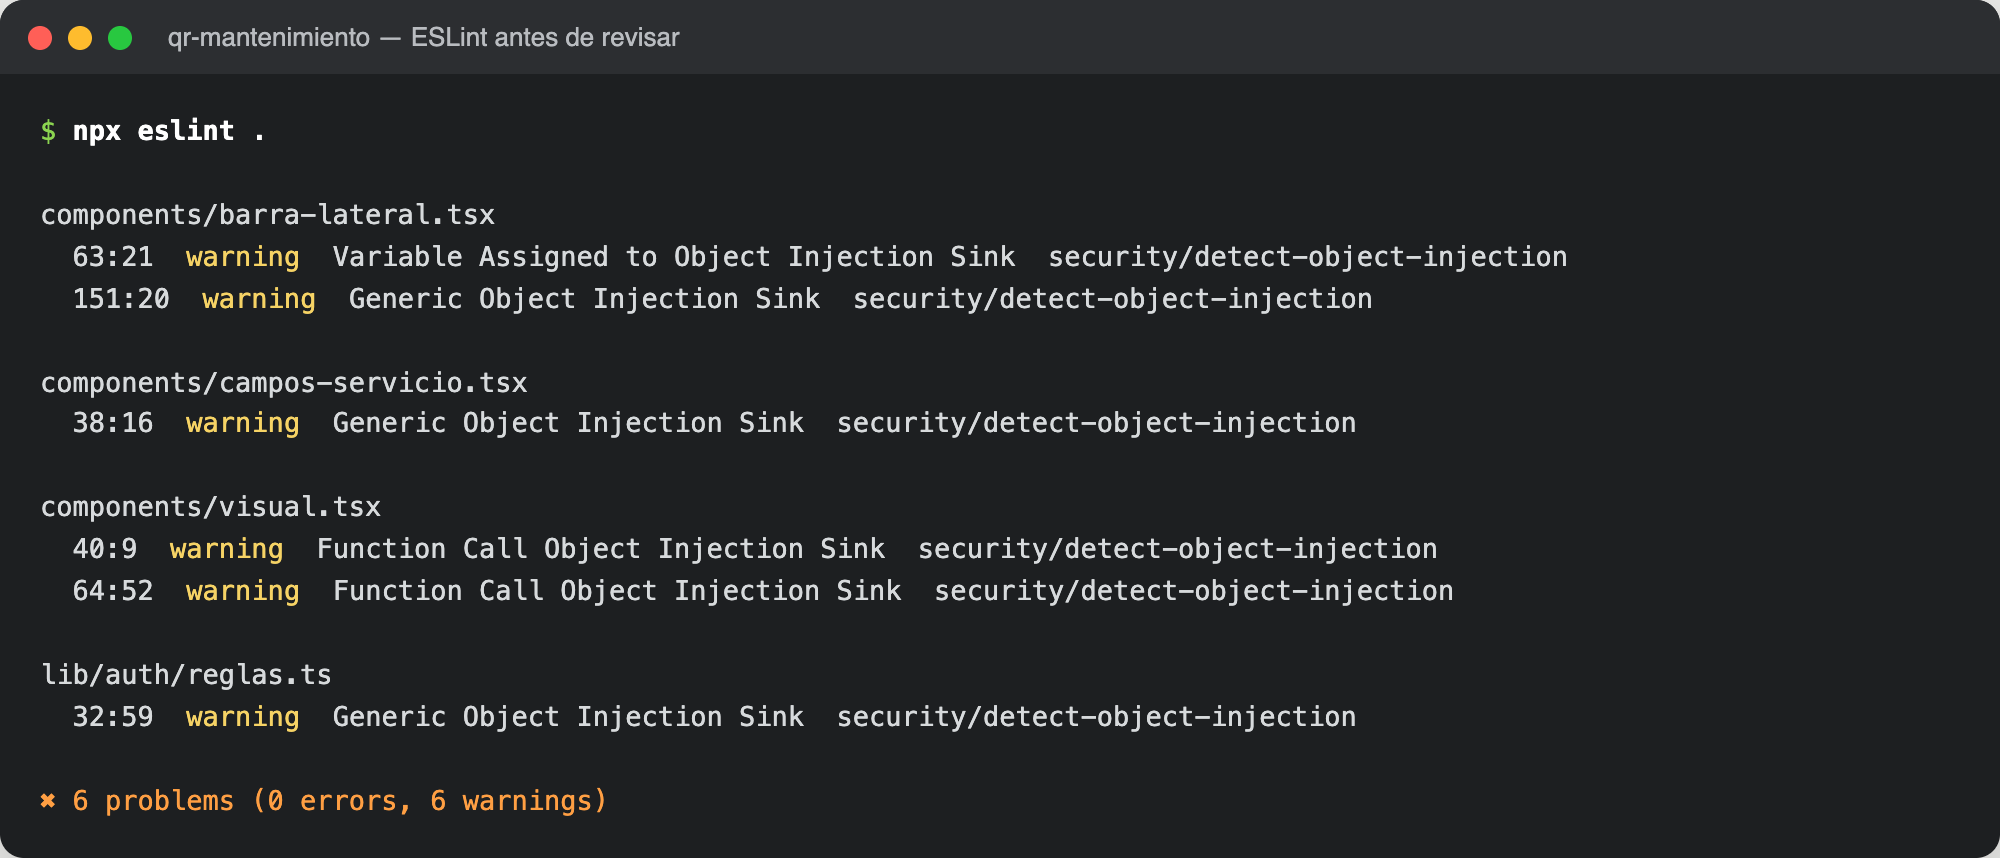
\includegraphics[width=\linewidth]{img/04-eslint-inicial.png}
  \caption{Resultado inicial de ESLint con las reglas de seguridad.}
  \label{fig:eslint-inicial}
\end{figure}

Revisamos los seis casos uno por uno y concluimos que son falsos positivos. En todos la clave tiene un tipo cerrado, como el rol del usuario o el tipo de servicio, y nunca viene directamente de una petición: el rol sale de la sesión y los tipos se validan antes con Zod. Para no ignorar la regla por completo, marcamos cada caso en el código con un comentario que explica la razón. Así el análisis queda limpio y cualquier aviso nuevo se nota de inmediato (figura \ref{fig:eslint-final}).

\begingroup\small\setlength{\tabcolsep}{4pt}\renewcommand{\arraystretch}{1.25}
\begin{longtable}{L{0.36}L{0.08}L{0.25}L{0.24}}
\toprule
\textbf{Archivo} & \textbf{Línea} & \textbf{Código} & \textbf{Clasificación} \\
\midrule
\endfirsthead
\toprule
\textbf{Archivo} & \textbf{Línea} & \textbf{Código} & \textbf{Clasificación} \\
\midrule
\endhead
\bottomrule
\endfoot
\nolinkurl{components/barra-lateral.tsx} & 63 & \texttt{SECCIONES[rol]} & Falso positivo \\
\nolinkurl{components/barra-lateral.tsx} & 151 & \texttt{NOMBRE\_DE\_ROL[rol]} & Falso positivo \\
\nolinkurl{components/campos-servicio.tsx} & 38 & \texttt{NOMBRE\_DE\_TIPO[valor]} & Falso positivo \\
\nolinkurl{components/visual.tsx} & 40 & \texttt{TONOS[tono]} & Falso positivo \\
\nolinkurl{components/visual.tsx} & 64 & \texttt{PUNTOS[tono]} & Falso positivo \\
\nolinkurl{lib/auth/reglas.ts} & 32 & \texttt{PLAZOS[rol]} & Falso positivo \\
\end{longtable}
\endgroup

\begin{figure}[H]
  \centering
  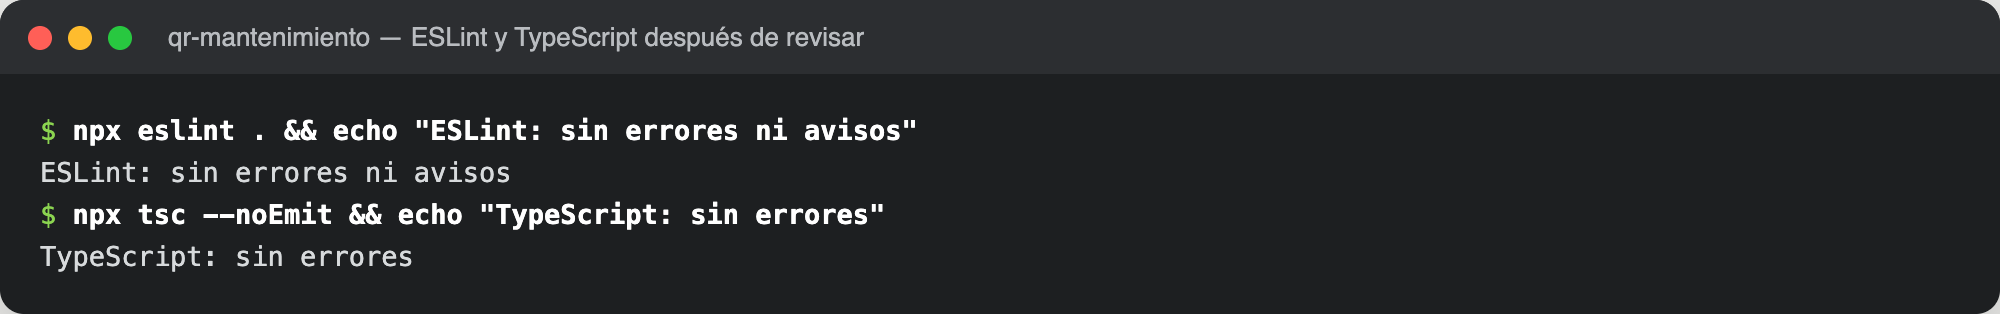
\includegraphics[width=\linewidth]{img/04-eslint-final.png}
  \caption{ESLint y TypeScript sin errores ni avisos después de revisar los falsos positivos.}
  \label{fig:eslint-final}
\end{figure}

\subsection{Revisión de dependencias}

La revisión de dependencias fue más reveladora. npm audit reportó 17 paquetes vulnerables, de los cuales 2 son críticos, 4 altos y 11 moderados (figura \ref{fig:audit}). Al quedarnos solo con las dependencias de producción el número baja a 8, con 4 altos y 4 moderados (figura \ref{fig:audit-prod}).

\begin{figure}[H]
  \centering
  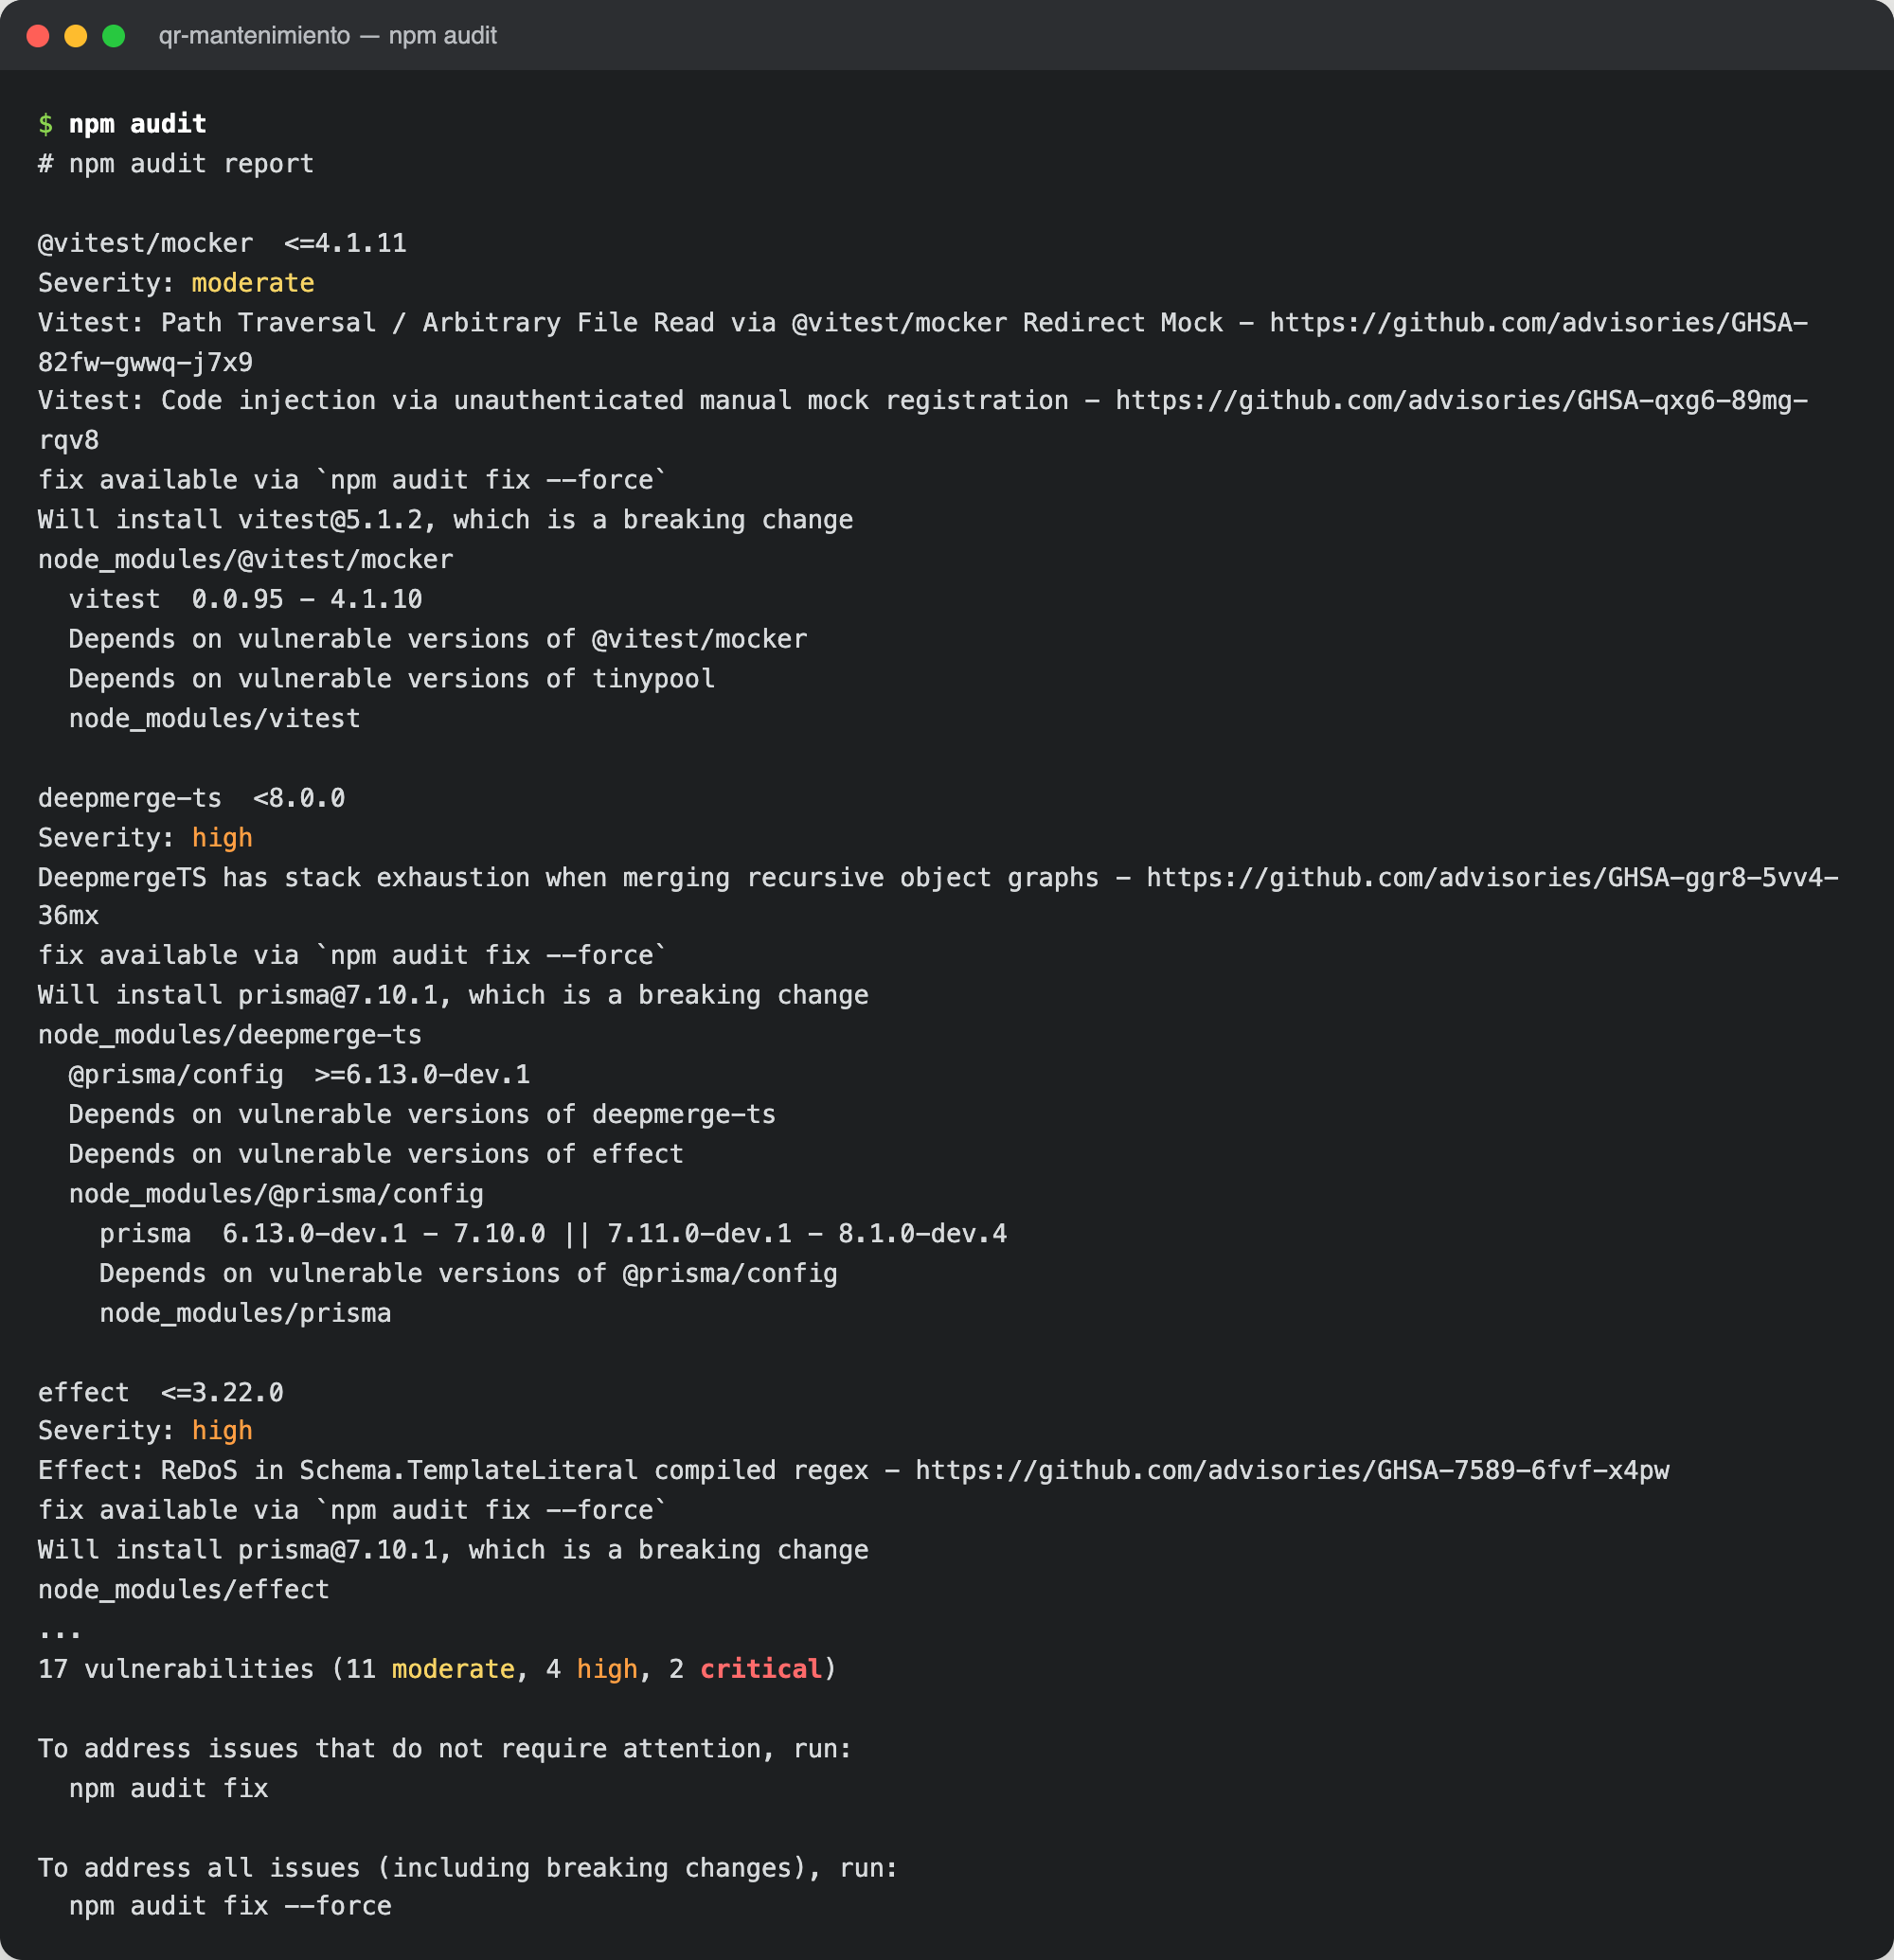
\includegraphics[width=\linewidth]{img/04-npm-audit.png}
  \caption{Inicio y resumen del reporte de npm audit sobre todas las dependencias.}
  \label{fig:audit}
\end{figure}

\begin{figure}[H]
  \centering
  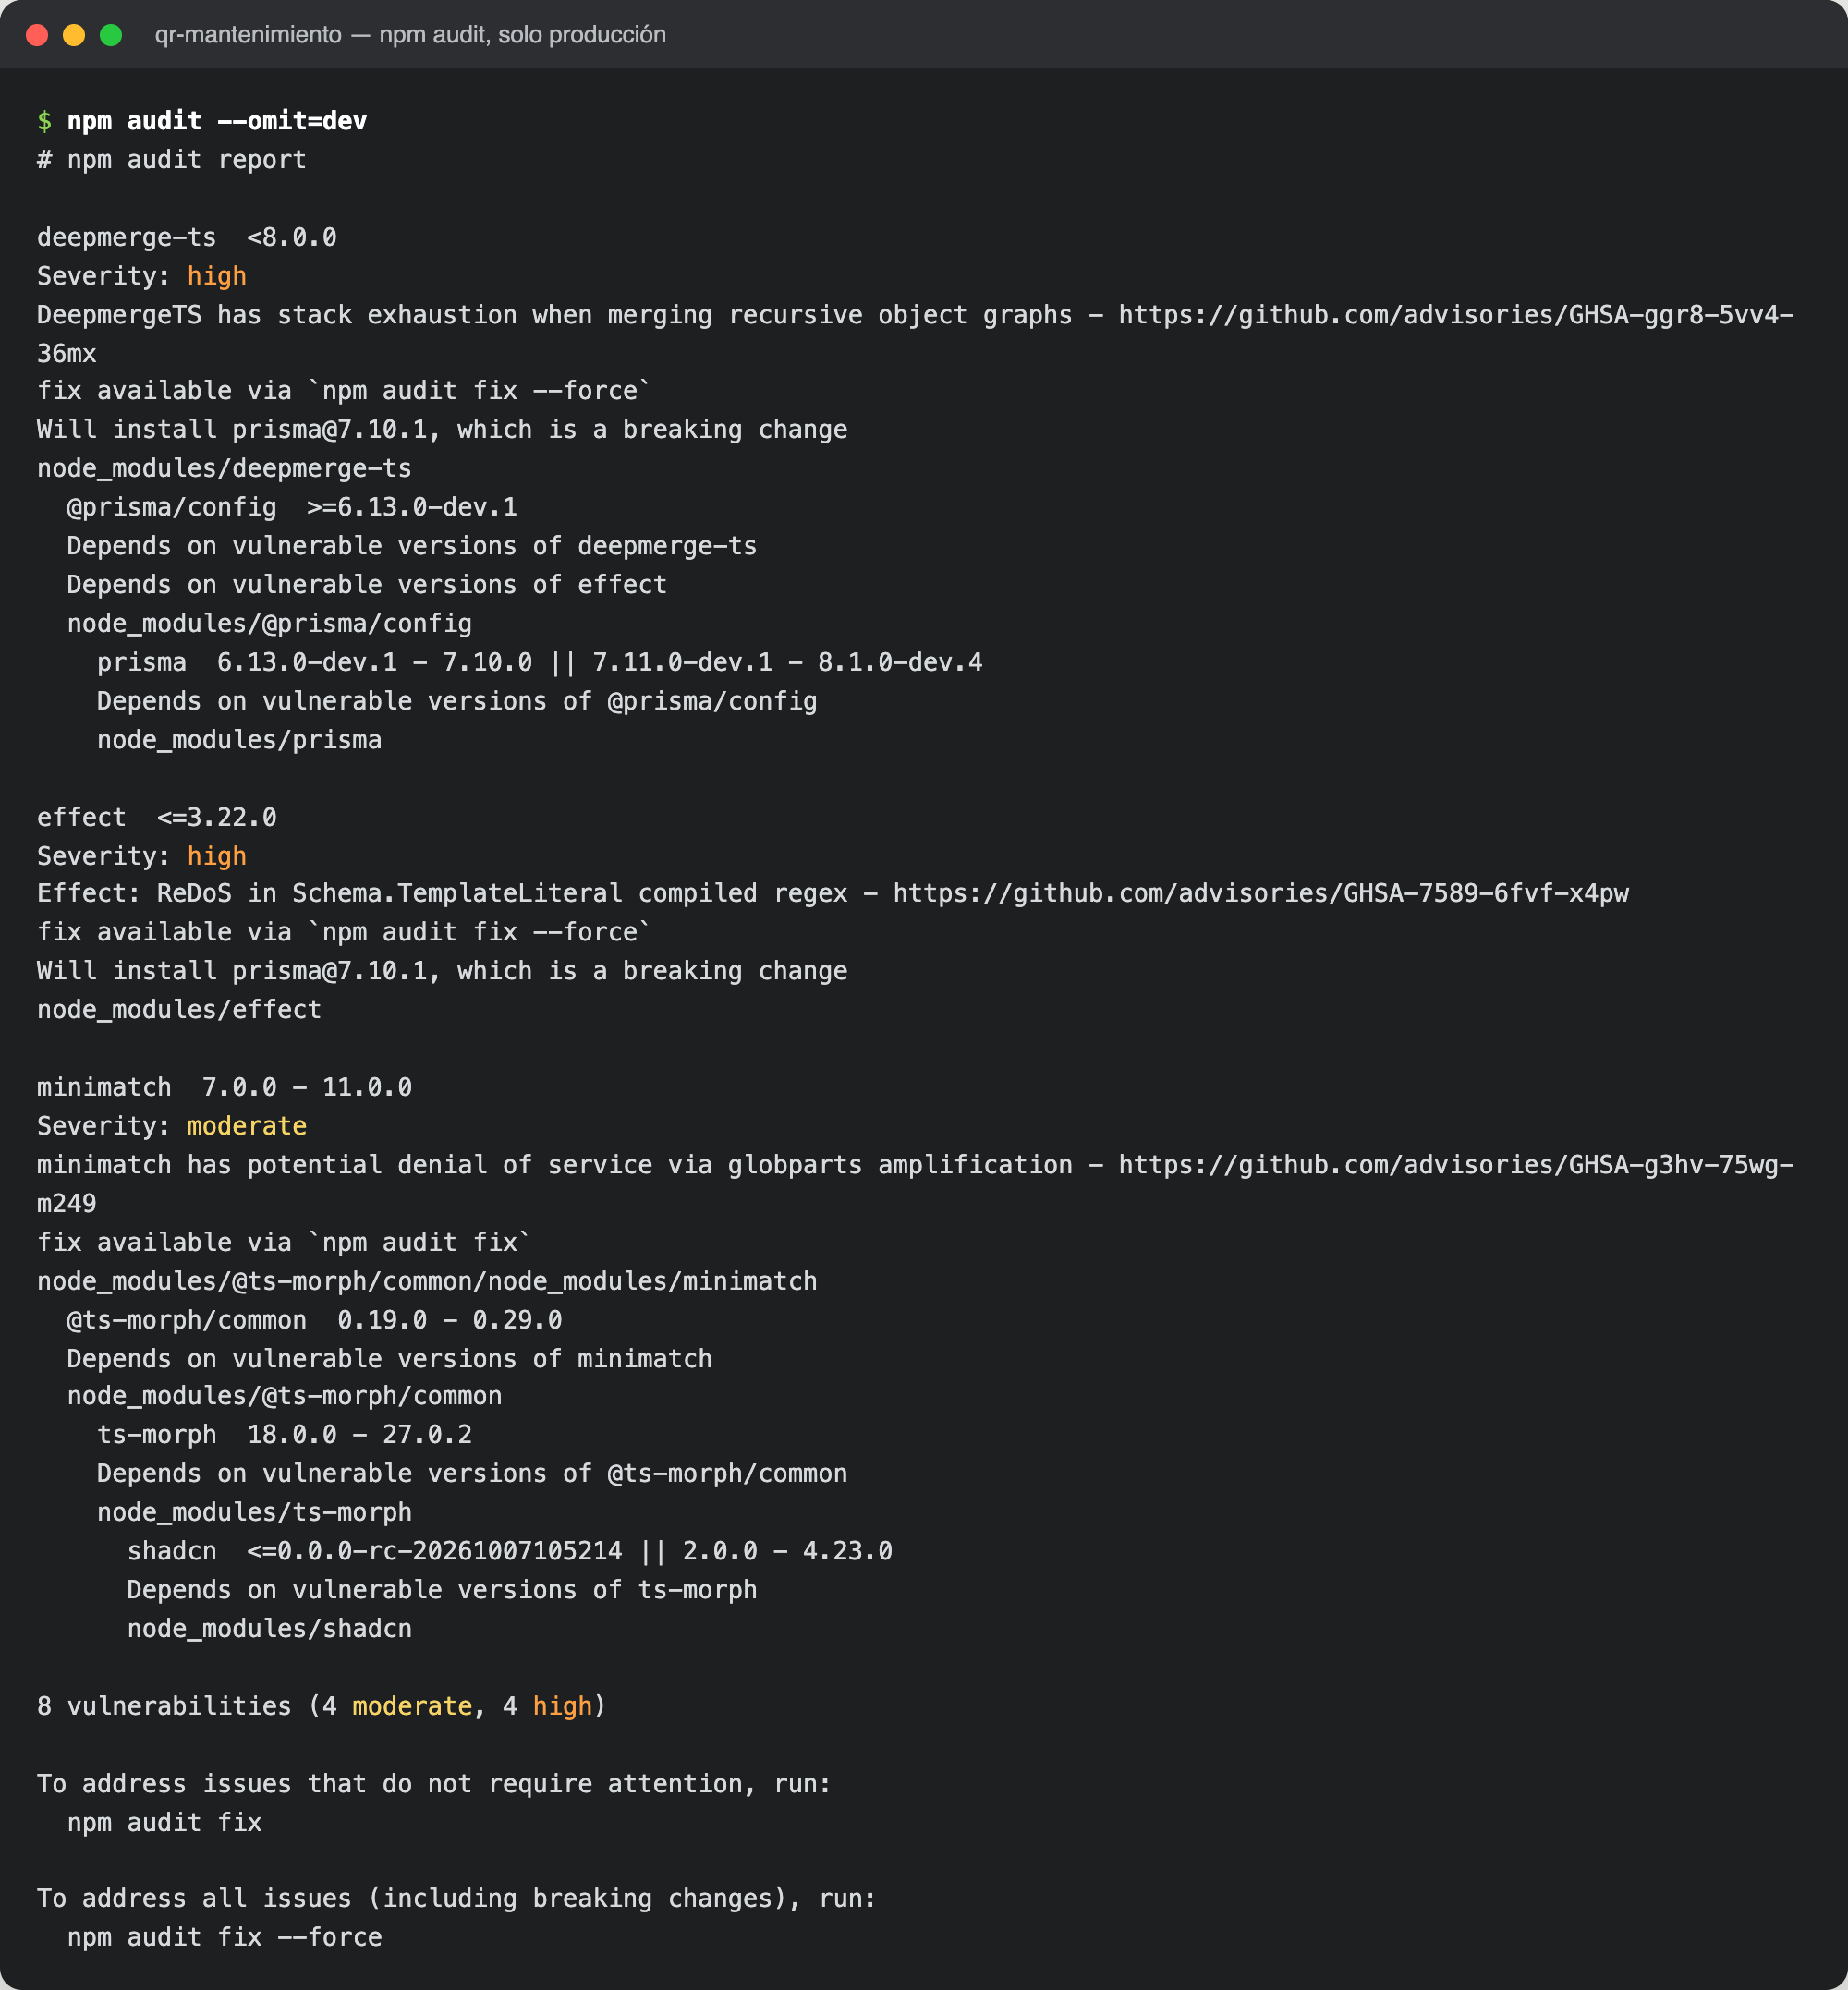
\includegraphics[width=\linewidth]{img/04-npm-audit-produccion.png}
  \caption{Reporte de npm audit solo sobre las dependencias de producción.}
  \label{fig:audit-prod}
\end{figure}

\begingroup\small\setlength{\tabcolsep}{4pt}\renewcommand{\arraystretch}{1.25}
\begin{longtable}{L{0.17}L{0.11}L{0.11}L{0.24}L{0.13}L{0.14}}
\toprule
\textbf{Paquete} & \textbf{Versión} & \textbf{Severidad} & \textbf{Aviso} & \textbf{Llega por} & \textbf{Alcance} \\
\midrule
\endfirsthead
\toprule
\textbf{Paquete} & \textbf{Versión} & \textbf{Severidad} & \textbf{Aviso} & \textbf{Llega por} & \textbf{Alcance} \\
\midrule
\endhead
\bottomrule
\endfoot
tinypool & 1.1.1 & Crítica & GHSA-5gmw-xhrv-c9v3, GHSA-85c8-ppgw-ccpr & vitest & Desarrollo \\
vitest y @vitest/mocker & 3.2.7 & Moderada & GHSA-82fw-gwwq-j7x9, GHSA-qxg6-89mg-rqv8 & Directa & Desarrollo \\
deepmerge-ts & 7.1.5 & Alta & GHSA-ggr8-5vv4-36mx & prisma & Producción \\
effect & 3.21.0 & Alta & GHSA-7589-6fvf-x4pw & prisma & Producción \\
prisma y @prisma/config & 6.19.3 & Alta & Por las dos anteriores & Directa & Producción \\
minimatch & 7 a 11.0.0 & Moderada & GHSA-g3hv-75wg-m249 & shadcn y typescript-eslint & Ambos \\
shadcn y ts-morph & 4.23.0 & Moderada & Por minimatch & Directa & Producción \\
typescript-eslint & 8 & Moderada & Por minimatch & eslint-config-next & Desarrollo \\
\end{longtable}
\endgroup

Al analizar de dónde venía cada vulnerabilidad notamos tres cosas. Primero, las dos críticas están en \texttt{tinypool}, que solo usa el ejecutor de pruebas, así que no llegan a la aplicación en producción, aunque sí afectan al equipo de quien corre las pruebas y al servidor de integración continua. Segundo, \texttt{prisma} aparece en producción porque el cliente de Prisma lo pide como dependencia, pero las vulnerabilidades altas están en la configuración de su herramienta de línea de comandos y no en el cliente que corre dentro de la aplicación. Tercero, \texttt{shadcn} es una herramienta que solo usamos para agregar componentes y que, por error, quedó instalada como dependencia de producción.

\subsection{Hallazgos de la revisión manual}

Además de las herramientas, revisamos a mano las partes más sensibles del código, en especial la autorización, las sesiones y el uso de datos que llegan en la petición. Encontramos dos problemas que ninguna herramienta había señalado.

El primero, H-01, está en la función que obtiene la dirección IP del cliente (figura \ref{fig:h01}). La toma de la cabecera \texttt{X-Forwarded-For} sin comprobar que la haya puesto un proxy de confianza. Como cualquier cliente puede enviar esa cabecera con el valor que quiera, un atacante podría cambiar su IP en cada intento para esquivar el límite de intentos por dirección IP, y además dejaría direcciones falsas en la bitácora.

\begin{figure}[H]
  \centering
  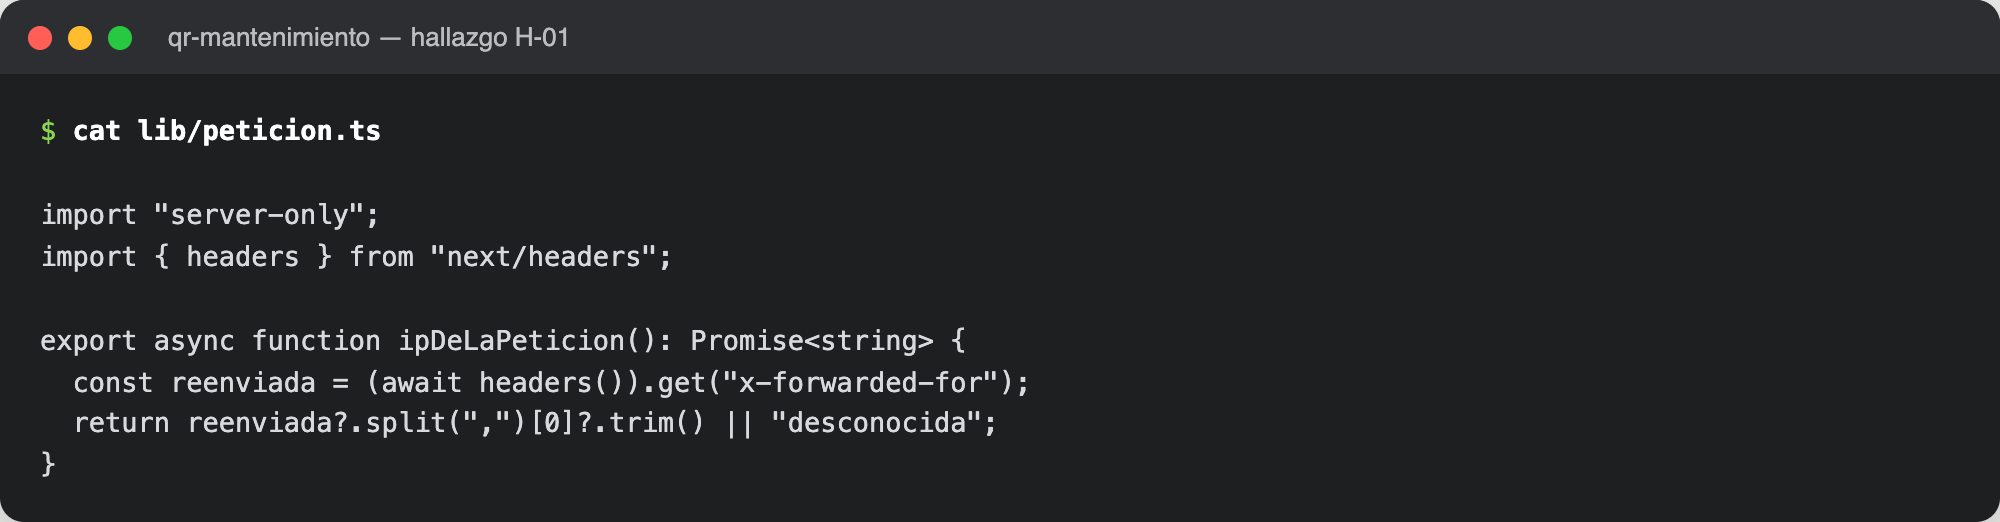
\includegraphics[width=\linewidth]{img/04-hallazgo-h01-ip.png}
  \caption{H-01. La IP se toma de una cabecera que controla el cliente.}
  \label{fig:h01}
\end{figure}

El segundo, H-02, está en la función que quita una asignación (figura \ref{fig:h02}). La pantalla solo permite quitar asignaciones de hoy en adelante, pero la función del servidor no revisa la fecha. Una petición hecha a mano podría borrar asignaciones de días pasados y alterar el registro de quién atendió cada equipo.

\begin{figure}[H]
  \centering
  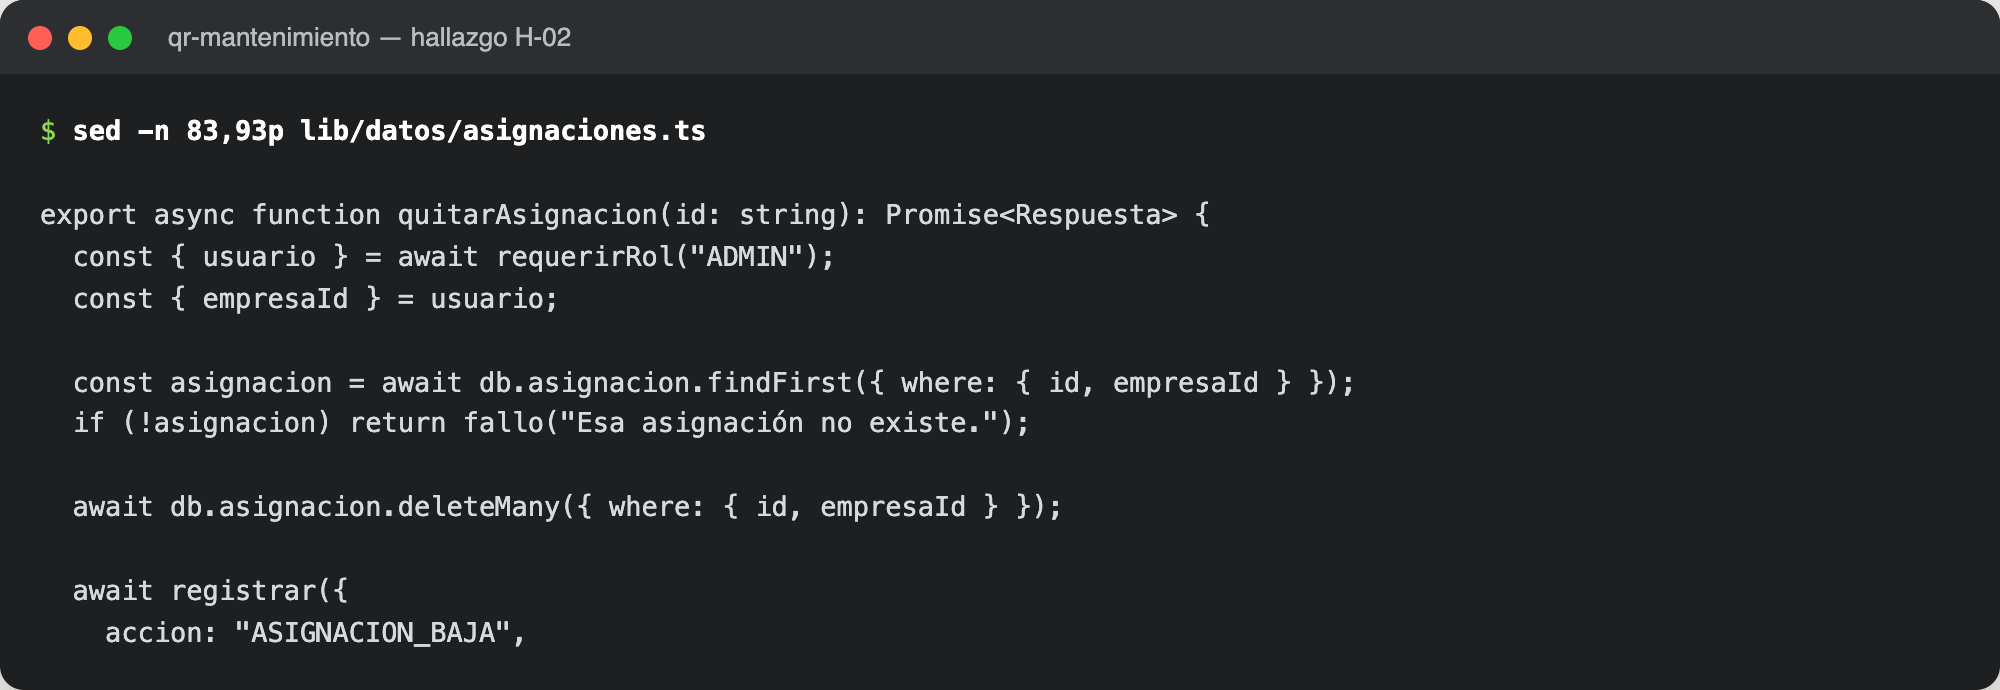
\includegraphics[width=\linewidth]{img/04-hallazgo-h02-asignaciones.png}
  \caption{H-02. La función que quita asignaciones no revisa la fecha.}
  \label{fig:h02}
\end{figure}

\begingroup\small\setlength{\tabcolsep}{4pt}\renewcommand{\arraystretch}{1.25}
\begin{longtable}{L{0.08}L{0.52}L{0.20}L{0.13}}
\toprule
\textbf{ID} & \textbf{Hallazgo} & \textbf{Origen} & \textbf{Severidad} \\
\midrule
\endfirsthead
\toprule
\textbf{ID} & \textbf{Hallazgo} & \textbf{Origen} & \textbf{Severidad} \\
\midrule
\endhead
\bottomrule
\endfoot
H-01 & La IP del cliente se toma de una cabecera que el cliente puede falsificar. & Revisión manual & Media \\
H-02 & Se pueden quitar asignaciones de días pasados con una petición hecha a mano. & Revisión manual & Baja \\
H-03 & Una herramienta de desarrollo, shadcn, está instalada como dependencia de producción. & npm audit & Baja \\
H-04 & Hay 17 dependencias con vulnerabilidades conocidas, dos de ellas críticas. & npm audit & Alta \\
\end{longtable}
\endgroup

Estos cuatro hallazgos pasan al registro de vulnerabilidades de la sección 5, donde se clasifican con detalle. Antes de corregirlos los confirmamos con pruebas dinámicas, que se describen en la sección 4.

% ─────────────────────────────────────────────────────────────────────────────
\section{4. Pruebas dinámicas de seguridad}

Las pruebas dinámicas atacan el sistema mientras está funcionando, para comprobar con hechos que las defensas del diseño se comportan como esperábamos. A diferencia del análisis estático, aquí no revisamos el código sino lo que responde el sistema cuando alguien intenta abusar de él.

\subsection{Entorno y método}

Para no alterar la base de datos de desarrollo, que guarda una bitácora que ya no se puede borrar, creamos una base exclusiva para las pruebas con las mismas dos empresas ficticias. Compilamos el sistema en modo de producción y lo levantamos en el puerto 3100. Las pruebas se ejecutan con un script que controla un navegador Chrome sin interfaz y que hace peticiones directas al servidor, de modo que se pueden repetir con los mismos pasos y comparar los resultados antes y después de cada corrección.

\begin{verbatim}
./scripts/preparar-pruebas.sh
npm run build
PORT=3100 DATABASE_URL=file:./pruebas.db npm start
node --env-file=.env scripts/pruebas-seguridad.mjs
\end{verbatim}

El script usa tres técnicas. Para las sesiones inicia sesión de verdad desde el navegador, igual que lo haría un usuario. Para atacar las acciones del servidor deja que la pantalla dispare una acción, la captura antes de que llegue y la vuelve a enviar con datos cambiados, que es lo mismo que podría hacer un atacante desde las herramientas de desarrollo del navegador. Para la inmutabilidad intenta modificar la base de datos directamente, sin pasar por la aplicación. Cada prueba compara el resultado obtenido con el esperado y lo marca como \textbf{Pasa} o \textbf{Falla}. Los resultados completos se guardan en \nolinkurl{evidencias/05-pruebas-dinamicas/resultados-inicial.json}.

\subsection{Resumen de resultados}

Ejecutamos 38 pruebas que cubren nueve de las once amenazas del modelo y los dos hallazgos de la revisión manual. Las amenazas T10 y T11, de dependencias y secretos, no se prueban atacando el sistema en funcionamiento, sino con el análisis de la sección 3 y con los controles de integración continua de la sección 8.

\begingroup\small\setlength{\tabcolsep}{4pt}\renewcommand{\arraystretch}{1.25}
\begin{longtable}{L{0.14}L{0.52}L{0.12}L{0.12}}
\toprule
\textbf{Amenaza} & \textbf{Qué se probó} & \textbf{Pasan} & \textbf{Fallan} \\
\midrule
\endfirsthead
\toprule
\textbf{Amenaza} & \textbf{Qué se probó} & \textbf{Pasan} & \textbf{Fallan} \\
\midrule
\endhead
\bottomrule
\endfoot
T1 & Enumeración de códigos QR & 2 & 0 \\
T2 & Acceso entre empresas, roles y equipos no asignados & 14 & 0 \\
T3 & Fuerza bruta y enumeración de cuentas & 2 & 0 \\
T4 & Cookies, revocación y cierre de sesión & 4 & 0 \\
T5 & Inyección, XSS y política CSP & 2 & 0 \\
T6 & Confirmación del equipo antes de registrar & 1 & 0 \\
T7 & Inmutabilidad de servicios y bitácora & 4 & 0 \\
T8 & Rutas y peticiones malformadas & 5 & 0 \\
T9 & Tope de reportes y tamaño de formularios & 2 & 0 \\
H-01 & IP falsificada con X-Forwarded-For & 0 & 1 \\
H-02 & Asignaciones de días pasados & 0 & 1 \\
\midrule
\textbf{Total} & & \textbf{36} & \textbf{2} \\
\end{longtable}
\endgroup

El resultado más importante es que todas las defensas del diseño original resistieron, incluida la matriz completa de autorización, y que las dos pruebas que fallan son justamente las que confirman los hallazgos de la revisión manual. Las figuras \ref{fig:pruebas-1} a \ref{fig:pruebas-4} muestran la salida completa del script.

\begin{figure}[H]
  \centering
  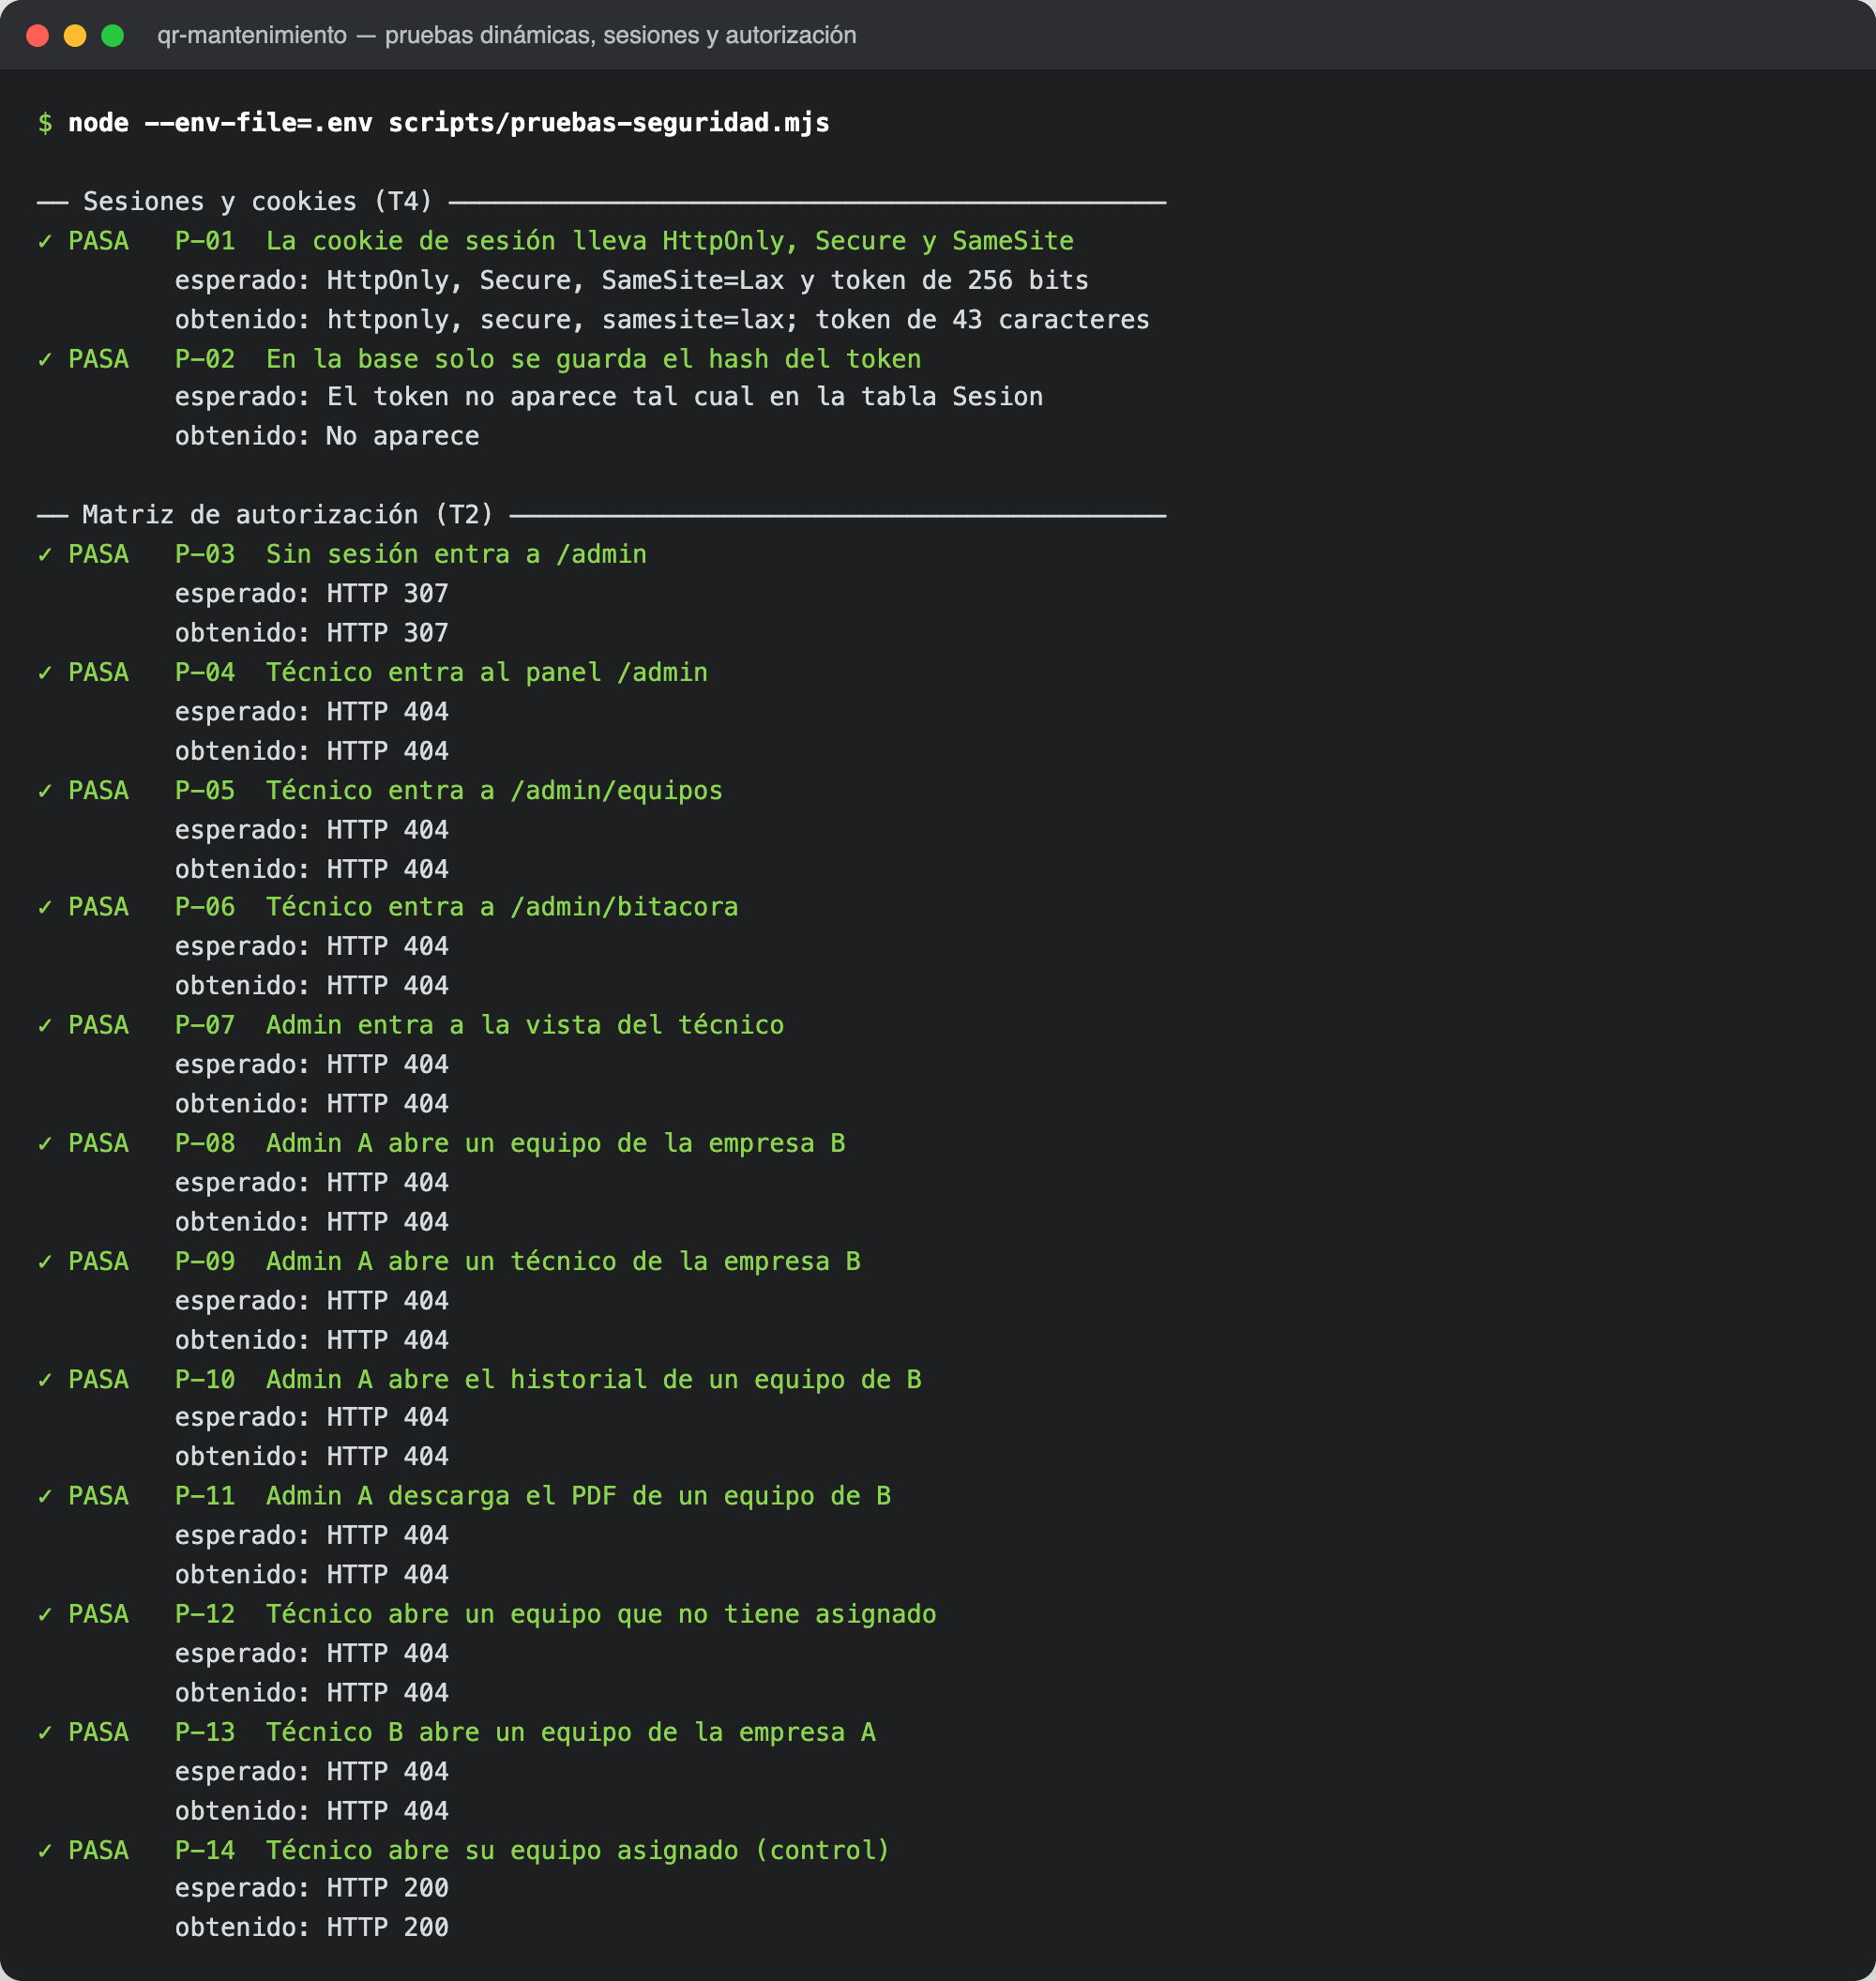
\includegraphics[width=\linewidth]{img/05-pruebas-1-autorizacion.png}
  \caption{Pruebas de sesiones, cookies y matriz de autorización.}
  \label{fig:pruebas-1}
\end{figure}

\begin{figure}[H]
  \centering
  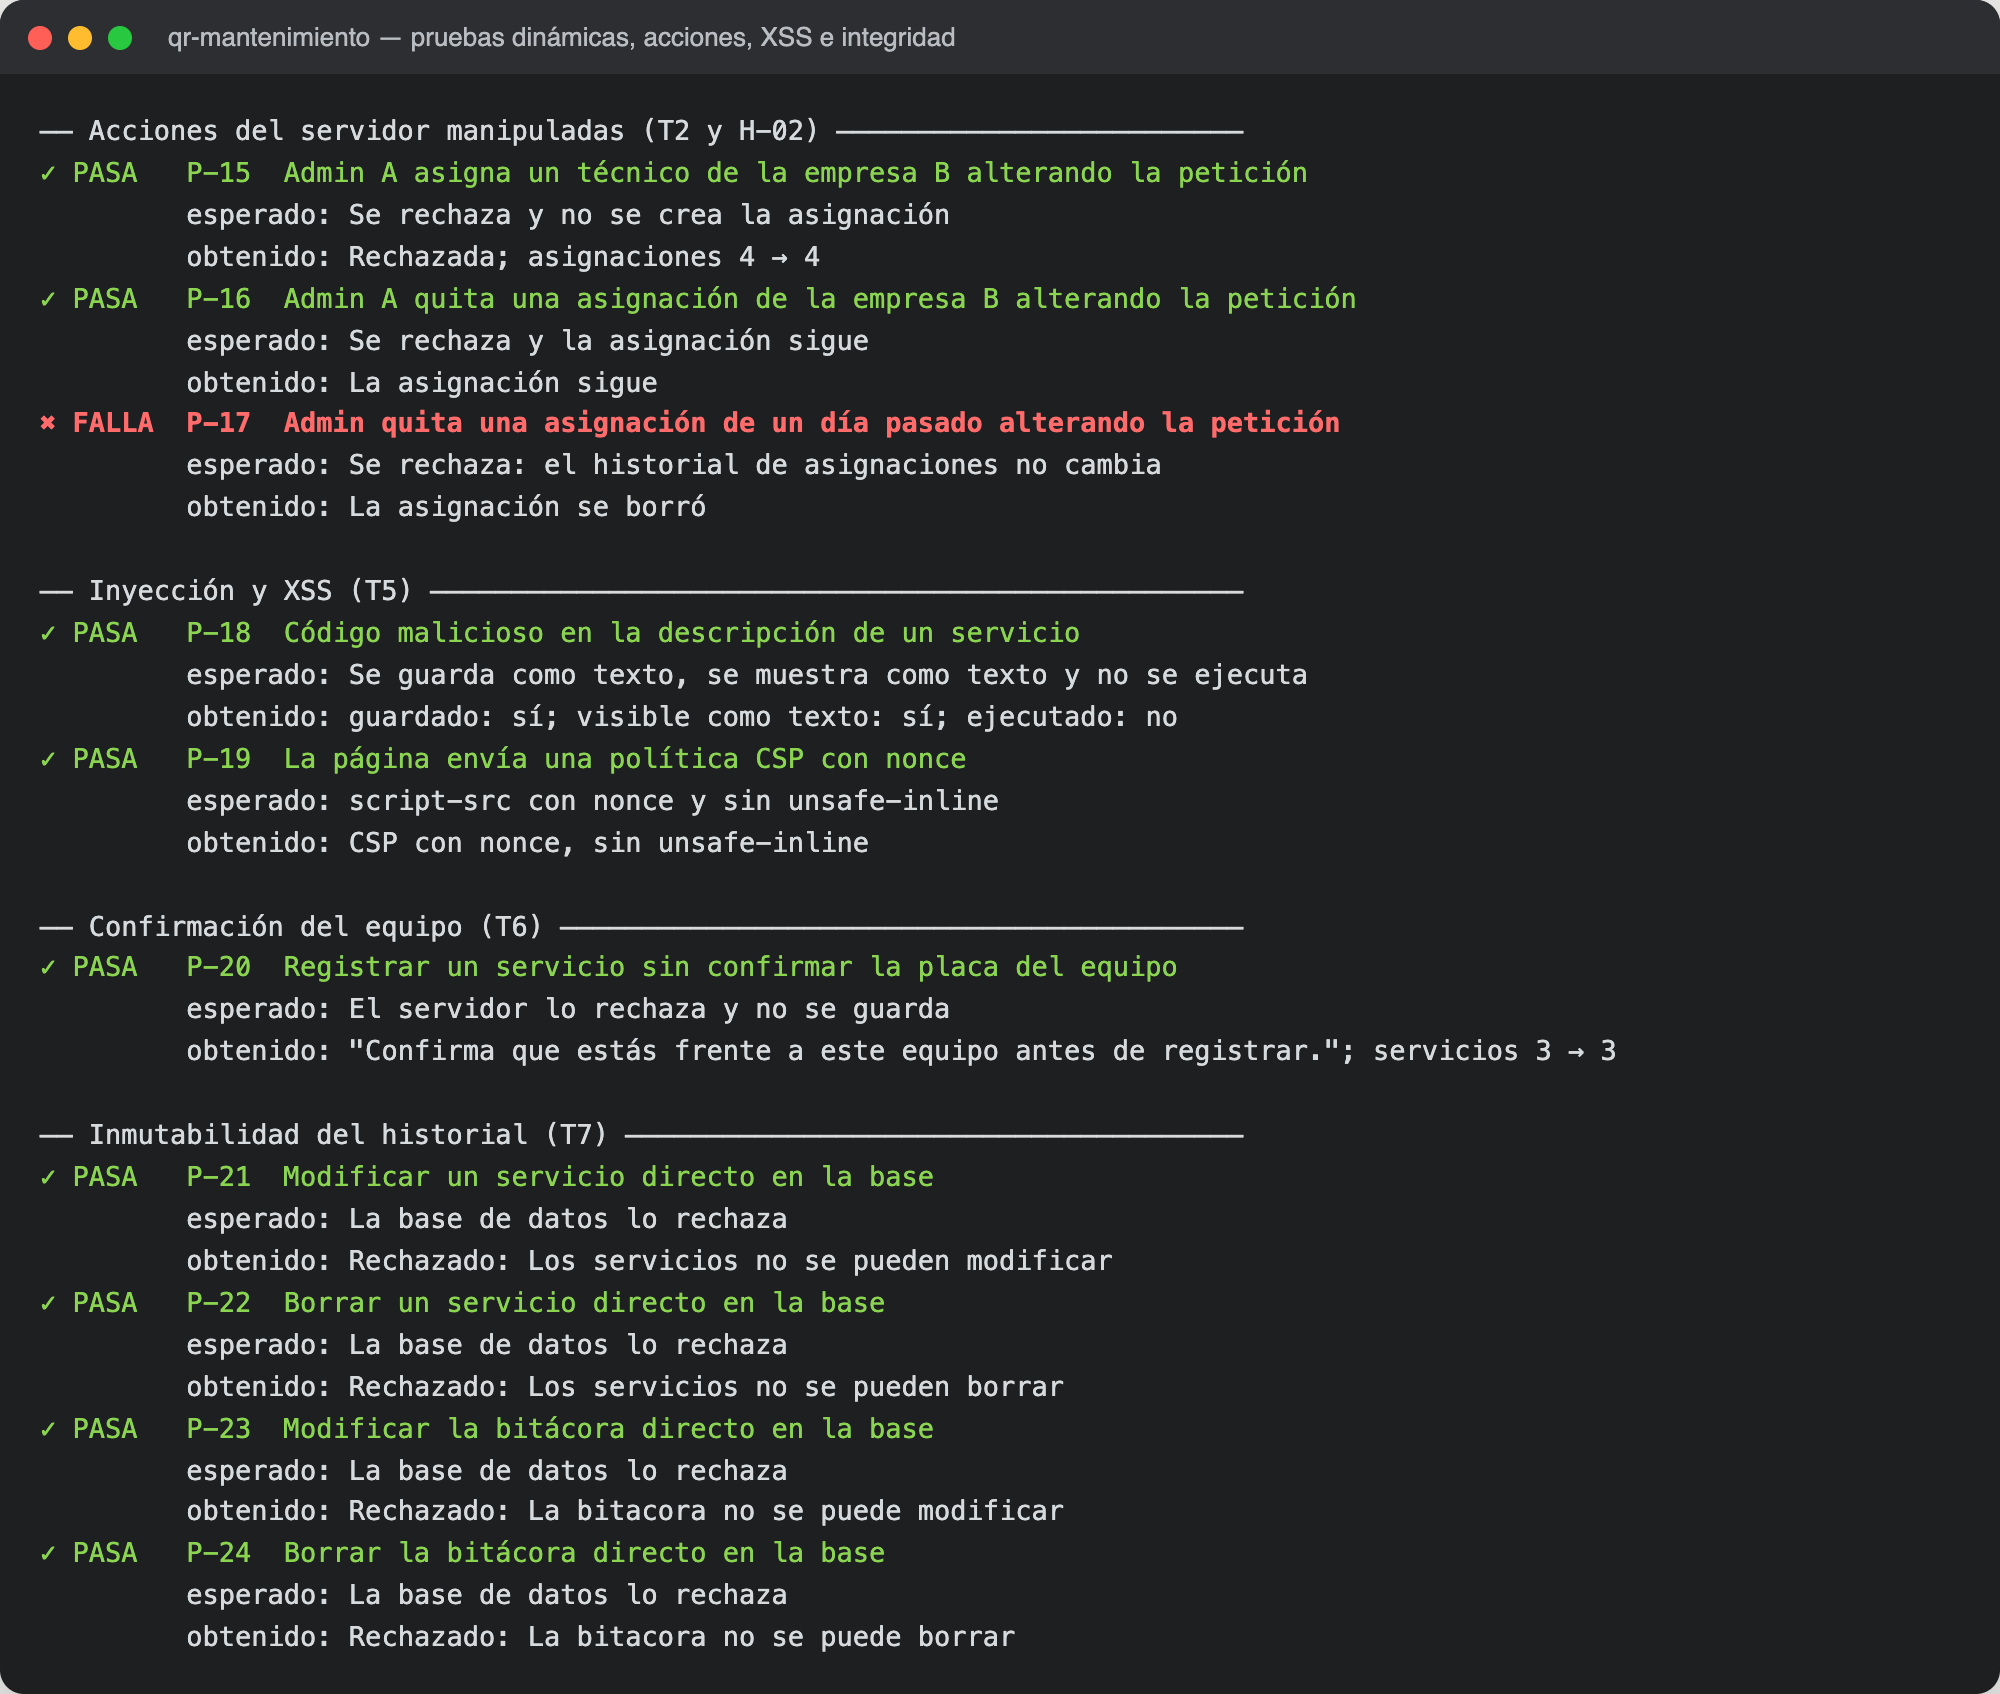
\includegraphics[width=\linewidth]{img/05-pruebas-2-acciones-xss.png}
  \caption{Pruebas de acciones manipuladas, XSS, confirmación del equipo e inmutabilidad.}
  \label{fig:pruebas-2}
\end{figure}

\begin{figure}[H]
  \centering
  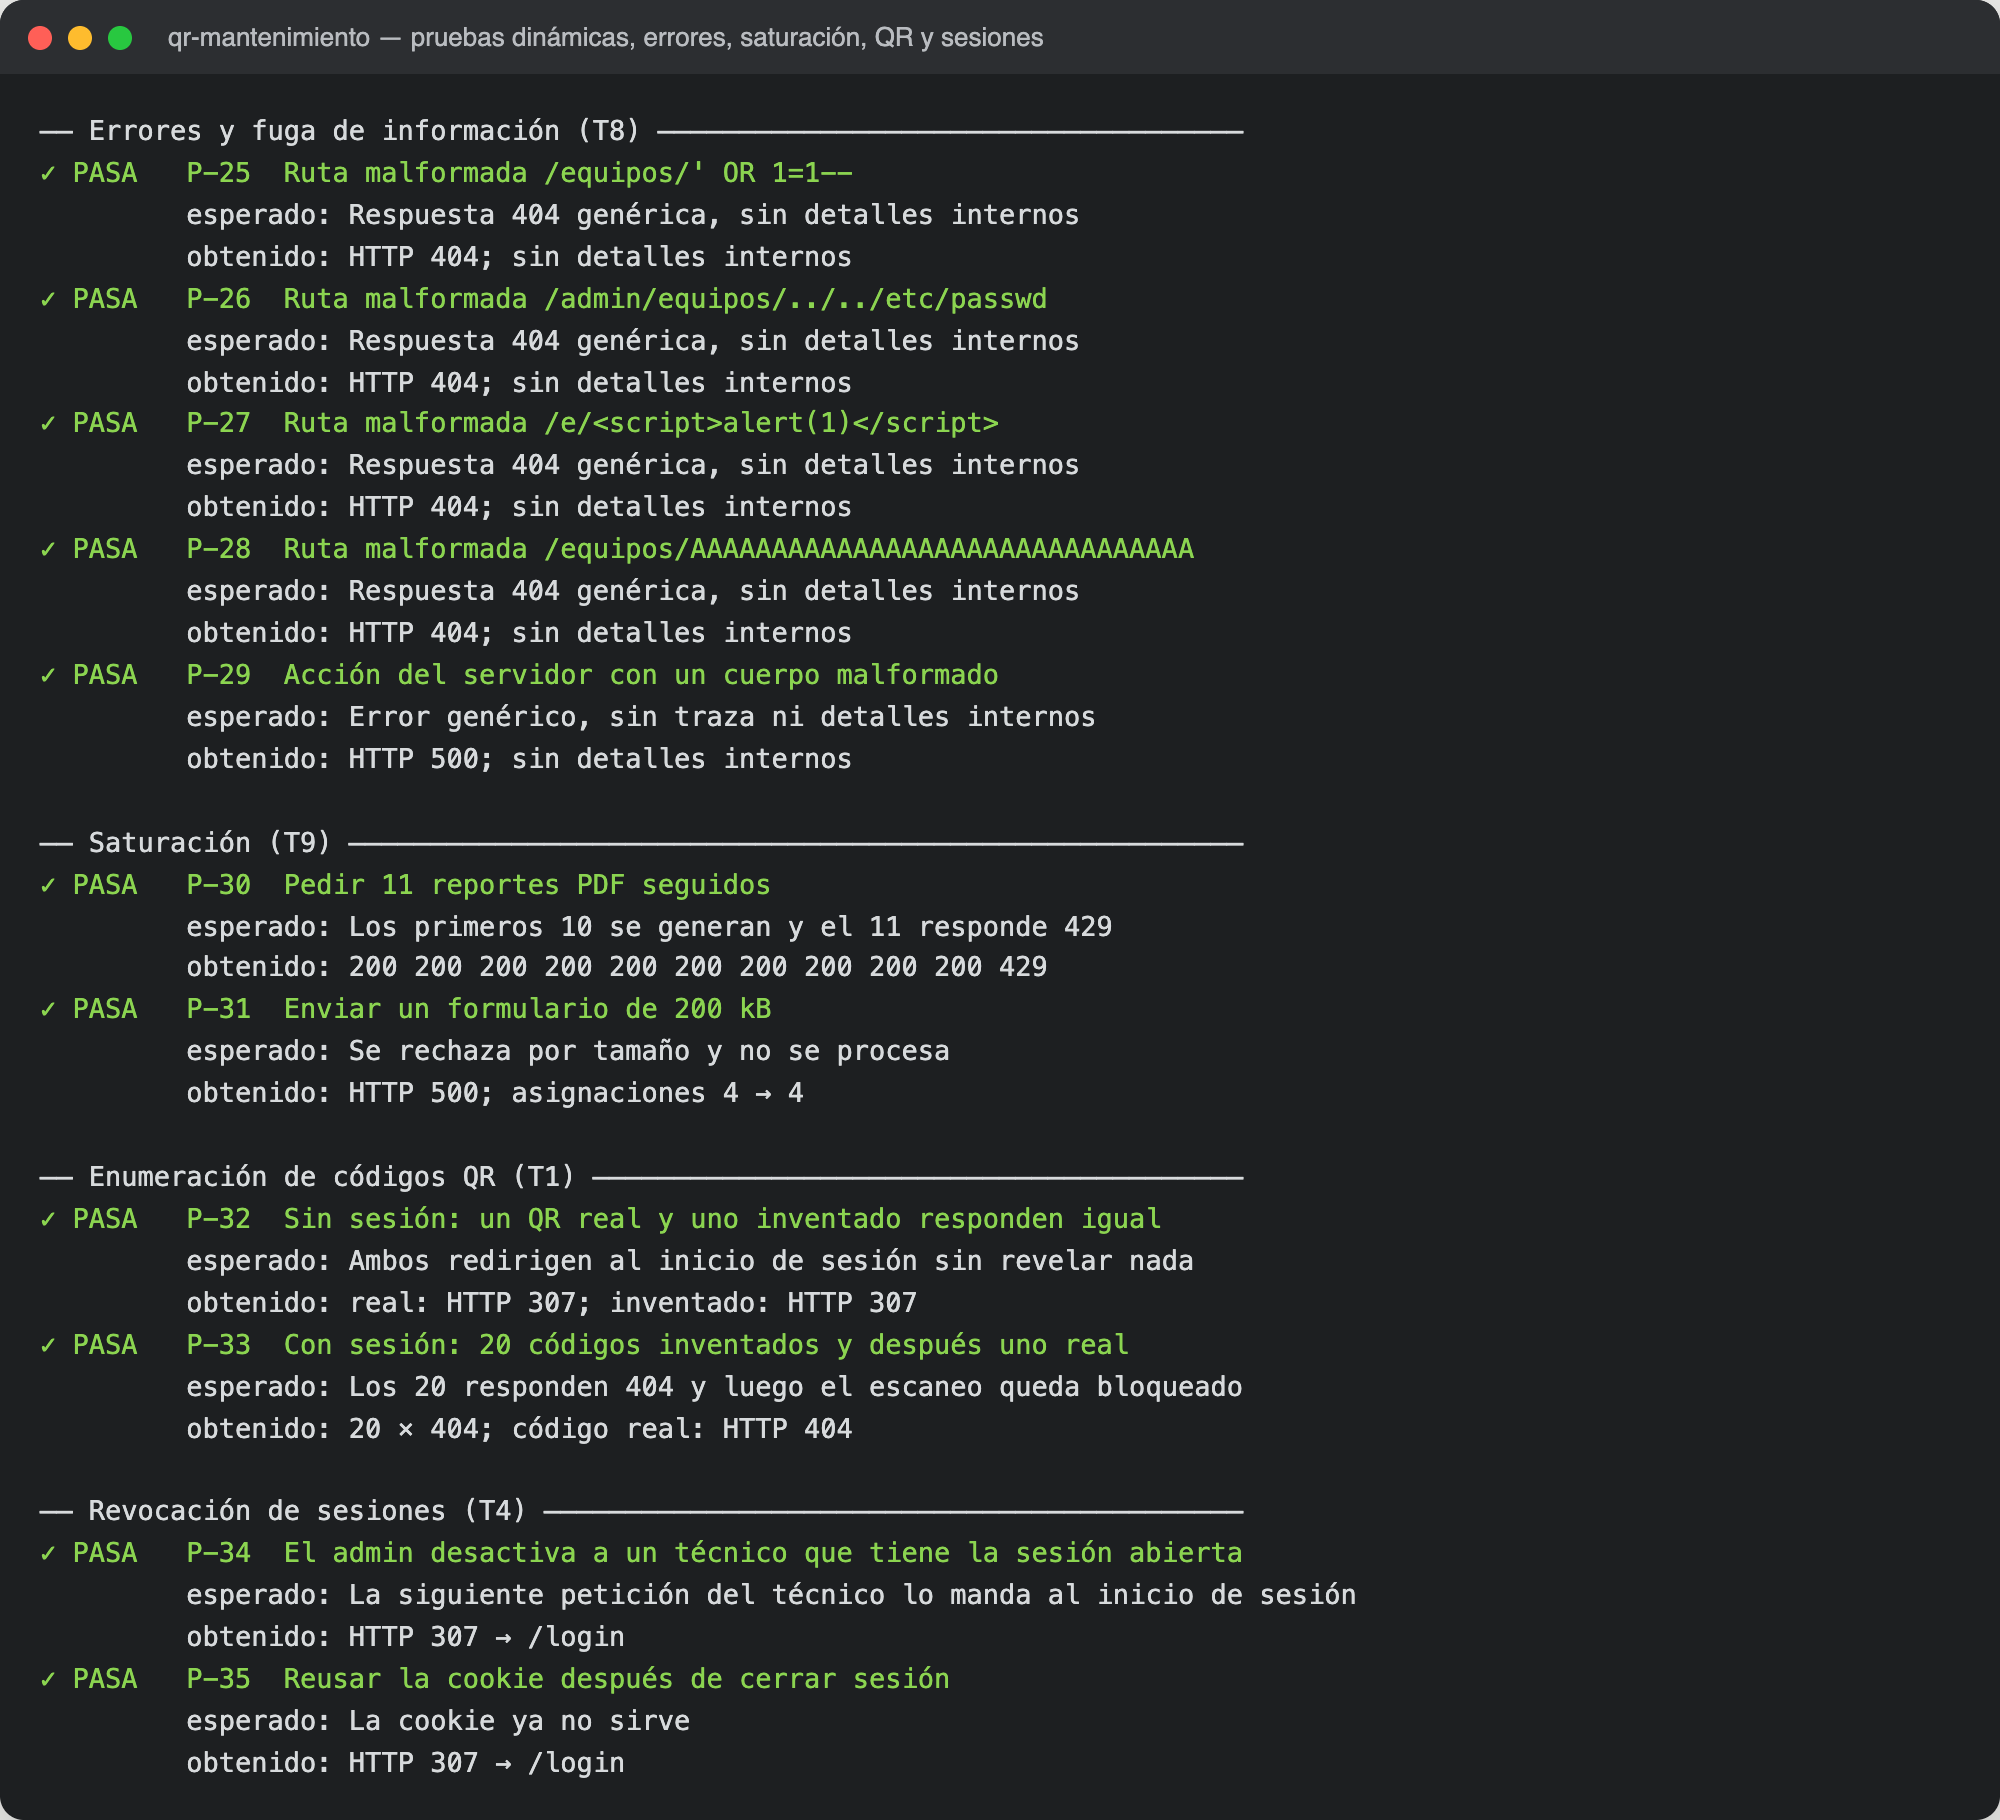
\includegraphics[width=\linewidth]{img/05-pruebas-3-errores-qr.png}
  \caption{Pruebas de errores, saturación, enumeración de QR y revocación de sesiones.}
  \label{fig:pruebas-3}
\end{figure}

\begin{figure}[H]
  \centering
  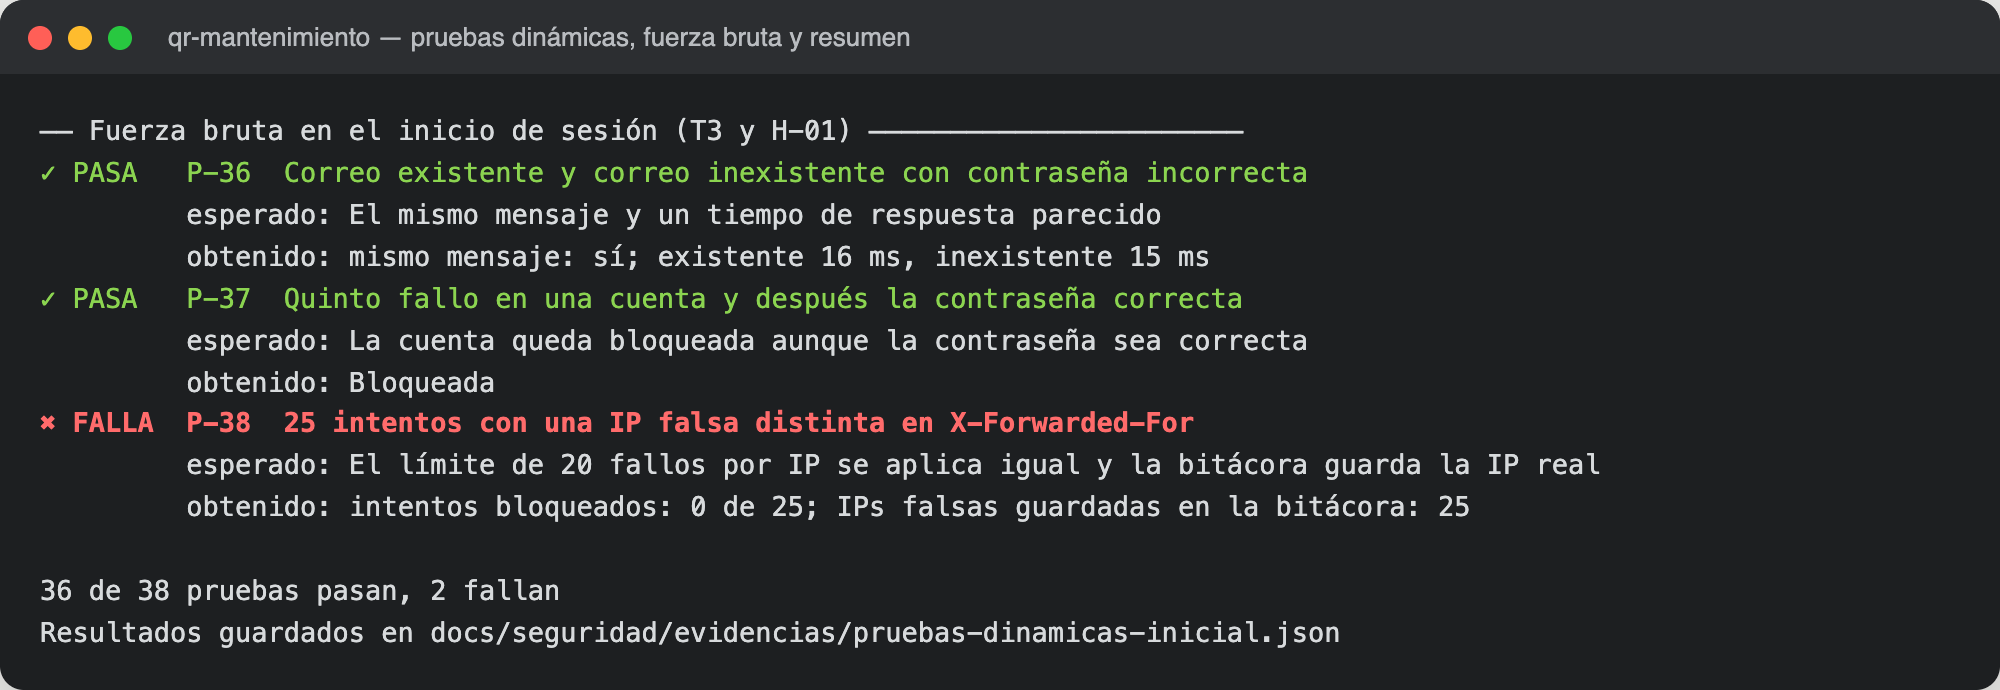
\includegraphics[width=\linewidth]{img/05-pruebas-4-fuerza-bruta.png}
  \caption{Pruebas de fuerza bruta y resumen final.}
  \label{fig:pruebas-4}
\end{figure}

\subsection{Detalle de las pruebas}

\begingroup\small\setlength{\tabcolsep}{4pt}\renewcommand{\arraystretch}{1.25}
\begin{longtable}{L{0.07}L{0.11}L{0.34}L{0.32}L{0.08}}
\toprule
\textbf{ID} & \textbf{Amenaza} & \textbf{Prueba} & \textbf{Resultado obtenido} & \textbf{Estado} \\
\midrule
\endfirsthead
\toprule
\textbf{ID} & \textbf{Amenaza} & \textbf{Prueba} & \textbf{Resultado obtenido} & \textbf{Estado} \\
\midrule
\endhead
\bottomrule
\endfoot
P-01 & T4 & La cookie de sesión lleva HttpOnly, Secure y SameSite & httponly, secure, samesite=lax; token de 43 caracteres & \textbf{Pasa} \\
P-02 & T4 & En la base solo se guarda el hash del token & No aparece & \textbf{Pasa} \\
P-03 & T2 & Sin sesión entra a /admin & HTTP 307 & \textbf{Pasa} \\
P-04 & T2 & Técnico entra al panel /admin & HTTP 404 & \textbf{Pasa} \\
P-05 & T2 & Técnico entra a /admin/equipos & HTTP 404 & \textbf{Pasa} \\
P-06 & T2 & Técnico entra a /admin/bitacora & HTTP 404 & \textbf{Pasa} \\
P-07 & T2 & Admin entra a la vista del técnico & HTTP 404 & \textbf{Pasa} \\
P-08 & T2 & Admin A abre un equipo de la empresa B & HTTP 404 & \textbf{Pasa} \\
P-09 & T2 & Admin A abre un técnico de la empresa B & HTTP 404 & \textbf{Pasa} \\
P-10 & T2 & Admin A abre el historial de un equipo de B & HTTP 404 & \textbf{Pasa} \\
P-11 & T2 & Admin A descarga el PDF de un equipo de B & HTTP 404 & \textbf{Pasa} \\
P-12 & T2 & Técnico abre un equipo que no tiene asignado & HTTP 404 & \textbf{Pasa} \\
P-13 & T2 & Técnico B abre un equipo de la empresa A & HTTP 404 & \textbf{Pasa} \\
P-14 & T2 & Técnico abre su equipo asignado (control) & HTTP 200 & \textbf{Pasa} \\
P-15 & T2 & Admin A asigna un técnico de la empresa B alterando la petición & Rechazada; asignaciones 4 $\rightarrow$ 4 & \textbf{Pasa} \\
P-16 & T2 & Admin A quita una asignación de la empresa B alterando la petición & La asignación sigue & \textbf{Pasa} \\
P-17 & H-02 & Admin quita una asignación de un día pasado alterando la petición & La asignación se borró & \textbf{\textcolor{red!70!black}{Falla}} \\
P-18 & T5 & Código malicioso en la descripción de un servicio & guardado: sí; visible como texto: sí; ejecutado: no & \textbf{Pasa} \\
P-19 & T5 & La página envía una política CSP con nonce & CSP con nonce, sin unsafe-inline & \textbf{Pasa} \\
P-20 & T6 & Registrar un servicio sin confirmar la placa del equipo & "Confirma que estás frente a este equipo antes de registrar."; servicios 3 $\rightarrow$ 3 & \textbf{Pasa} \\
P-21 & T7 & Modificar un servicio directo en la base & Rechazado: Los servicios no se pueden modificar & \textbf{Pasa} \\
P-22 & T7 & Borrar un servicio directo en la base & Rechazado: Los servicios no se pueden borrar & \textbf{Pasa} \\
P-23 & T7 & Modificar la bitácora directo en la base & Rechazado: La bitacora no se puede modificar & \textbf{Pasa} \\
P-24 & T7 & Borrar la bitácora directo en la base & Rechazado: La bitacora no se puede borrar & \textbf{Pasa} \\
P-25 & T8 & Ruta malformada /equipos/' OR 1=1-- & HTTP 404; sin detalles internos & \textbf{Pasa} \\
P-26 & T8 & Ruta malformada /admin/equipos/../../etc/passwd & HTTP 404; sin detalles internos & \textbf{Pasa} \\
P-27 & T8 & Ruta malformada /e/\textless{}script\textgreater{}alert(1)\textless{}/script\textgreater{} & HTTP 404; sin detalles internos & \textbf{Pasa} \\
P-28 & T8 & Ruta malformada /equipos/AAAAAAAAAAAAAAAAAAAAAAAAAAAAAAA & HTTP 404; sin detalles internos & \textbf{Pasa} \\
P-29 & T8 & Acción del servidor con un cuerpo malformado & HTTP 500; sin detalles internos & \textbf{Pasa} \\
P-30 & T9 & Pedir 11 reportes PDF seguidos & 200 200 200 200 200 200 200 200 200 200 429 & \textbf{Pasa} \\
P-31 & T9 & Enviar un formulario de 200 kB & HTTP 500; asignaciones 4 $\rightarrow$ 4 & \textbf{Pasa} \\
P-32 & T1 & Sin sesión: un QR real y uno inventado responden igual & real: HTTP 307; inventado: HTTP 307 & \textbf{Pasa} \\
P-33 & T1 & Con sesión: 20 códigos inventados y después uno real & 20 × 404; código real: HTTP 404 & \textbf{Pasa} \\
P-34 & T4 & El admin desactiva a un técnico que tiene la sesión abierta & HTTP 307 $\rightarrow$ /login & \textbf{Pasa} \\
P-35 & T4 & Reusar la cookie después de cerrar sesión & HTTP 307 $\rightarrow$ /login & \textbf{Pasa} \\
P-36 & T3 & Correo existente y correo inexistente con contraseña incorrecta & mismo mensaje: sí; existente 18 ms, inexistente 16 ms & \textbf{Pasa} \\
P-37 & T3 & Quinto fallo en una cuenta y después la contraseña correcta & Bloqueada & \textbf{Pasa} \\
P-38 & H-01 & 25 intentos con una IP falsa distinta en X-Forwarded-For & intentos bloqueados: 0 de 25; IPs falsas guardadas en la bitácora: 25 & \textbf{\textcolor{red!70!black}{Falla}} \\
\end{longtable}
\endgroup

\subsection{Hallazgos confirmados}

La prueba P-17 confirmó el hallazgo H-02. Capturamos la acción que quita una asignación de hoy, le cambiamos el identificador por el de una asignación de ayer y la reenviamos con la sesión del administrador. El servidor la aceptó y la asignación desapareció, aunque la pantalla nunca ofrece esa opción para días pasados. La defensa estaba solo en la interfaz y no en el servidor.

La prueba P-38 confirmó el hallazgo H-01 y mostró que su impacto es mayor de lo que estimamos. Hicimos 25 intentos de inicio de sesión fallidos, cada uno con una dirección IP inventada en la cabecera \texttt{X-Forwarded-For}. Ninguno se bloqueó, aunque el límite es de 20 fallos por dirección, y la bitácora guardó las 25 direcciones falsas como si fueran reales (figura \ref{fig:h01-bitacora}). Esto permite probar contraseñas contra muchas cuentas sin que el límite por IP lo detenga, y además le quita valor de evidencia a la bitácora, porque quien ataca decide qué dirección queda registrada.

\begin{figure}[H]
  \centering
  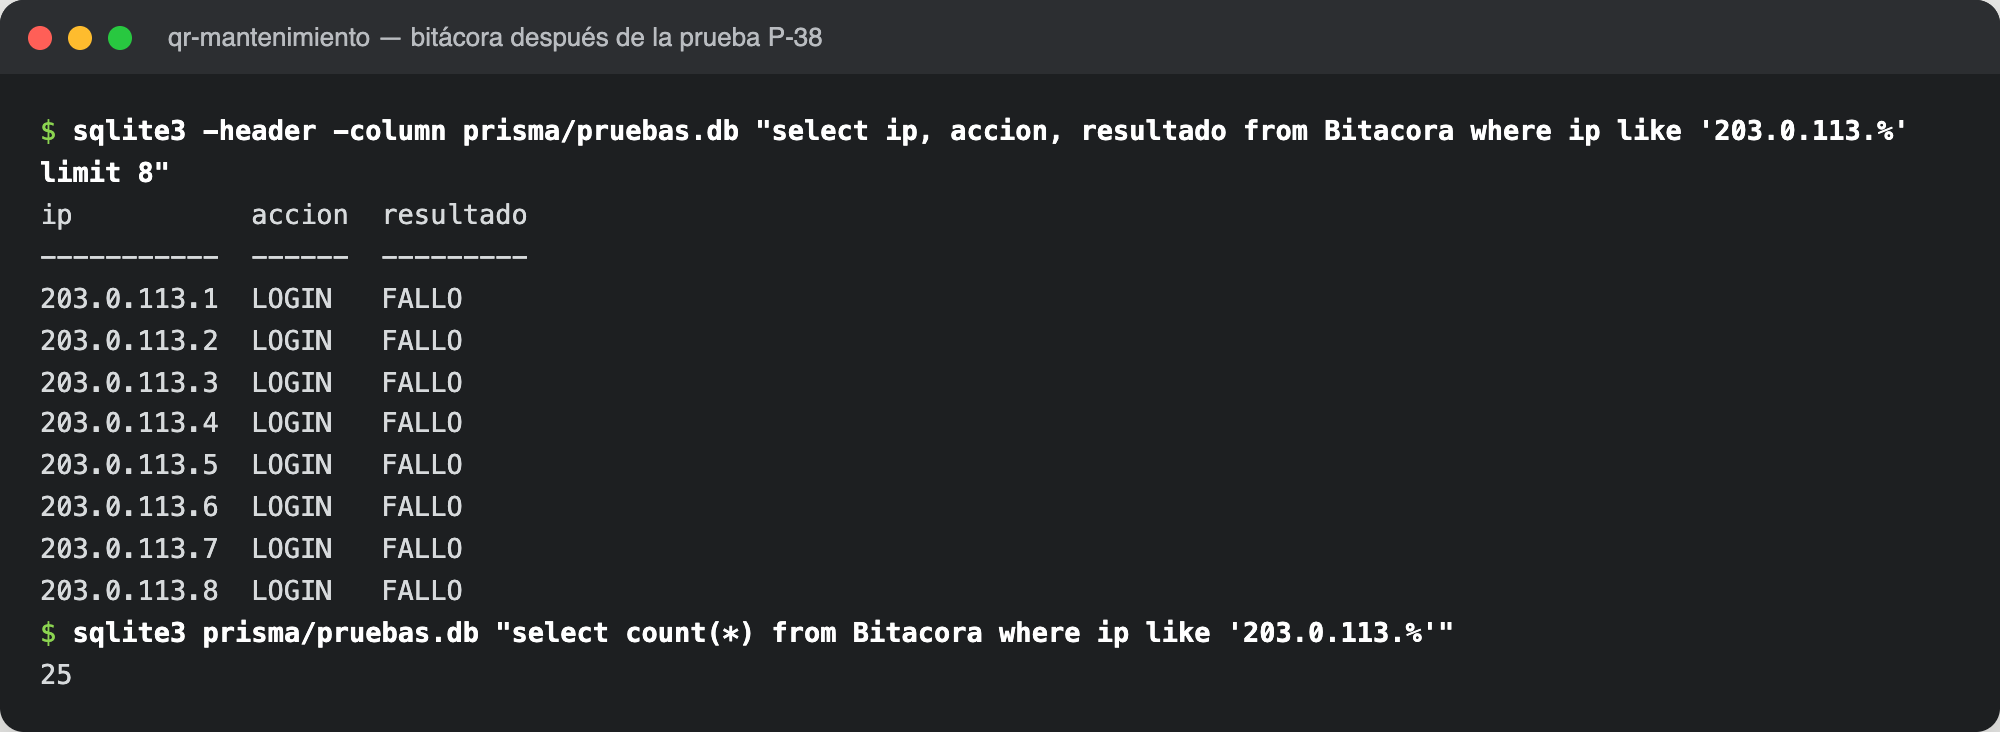
\includegraphics[width=\linewidth]{img/05-hallazgo-h01-bitacora.png}
  \caption{La bitácora guardó las 25 direcciones IP falsas de la prueba P-38.}
  \label{fig:h01-bitacora}
\end{figure}

\subsection{Observaciones}

En la prueba P-31 el formulario de 200 kB se rechazó como esperábamos y no se procesó, pero el servidor respondió con un error 500 en lugar del 413 que corresponde a un cuerpo demasiado grande. En el registro del servidor aparece el motivo real, \texttt{Body exceeded 100kb limit}. Como la respuesta no revela información y el límite sí funciona, lo registramos como observación de severidad informativa.

En la prueba P-36 los tiempos de respuesta con un correo existente y con uno inexistente fueron de 18 y 16 milisegundos. La diferencia es mínima porque, cuando el correo no existe, el sistema compara la contraseña contra un hash de relleno, así que el tiempo no delata qué cuentas existen.

\section{5. Registro y clasificación de vulnerabilidades}

En esta sección reunimos todo lo que encontramos en el análisis estático, la revisión de dependencias y las pruebas dinámicas, y lo clasificamos con el mismo criterio para decidir qué corregir primero. Registramos nueve hallazgos. Siete los corregimos, como se describe en la sección 6, y dos los aceptamos de forma justificada.

\subsection{Cómo los clasificamos}

Cada hallazgo se describe con su causa, su impacto y la evidencia que lo respalda, y se clasifica con tres referencias conocidas. La primera es CWE, el catálogo de tipos de debilidad de software que mantiene MITRE, que indica qué clase de error es. La segunda es el OWASP Top 10 de 2021, que lo ubica entre los riesgos más comunes en aplicaciones web. La tercera es STRIDE, la misma clasificación de amenazas que usamos en el primer entregable, para relacionarlo con nuestro modelo.

El nivel de riesgo lo calculamos igual que en el primer entregable, combinando la probabilidad de que alguien lo aproveche con el impacto que tendría en nuestro sistema, según la tabla siguiente.

\begin{center}
\small
\renewcommand{\arraystretch}{1.4}
\begin{tabular}{lccc}
\toprule
\textbf{Probabilidad} & \textbf{Impacto bajo} & \textbf{Impacto medio} & \textbf{Impacto alto} \\
\midrule
Alta  & \cellcolor{orange!30}Medio & \cellcolor{red!25}Alto & \cellcolor{red!25}Alto \\
Media & \cellcolor{yellow!25}Bajo & \cellcolor{orange!30}Medio & \cellcolor{red!25}Alto \\
Baja  & \cellcolor{yellow!25}Bajo & \cellcolor{yellow!25}Bajo & \cellcolor{orange!30}Medio \\
\bottomrule
\end{tabular}
\end{center}

Un hallazgo que no afecta a los datos ni a la disponibilidad lo marcamos como informativo. También distinguimos entre la severidad que publica cada aviso de seguridad y el riesgo real en nuestro sistema. Por ejemplo, la vulnerabilidad crítica de tinypool queda en riesgo medio porque solo se ejecuta durante las pruebas y nunca llega a producción.

\subsection{Resumen}

\begingroup\small\setlength{\tabcolsep}{4pt}\renewcommand{\arraystretch}{1.25}
\begin{longtable}{L{0.08}L{0.60}L{0.13}L{0.12}}
\toprule
\textbf{ID} & \textbf{Vulnerabilidad} & \textbf{Riesgo} & \textbf{Estado} \\
\midrule
\endfirsthead
\toprule
\textbf{ID} & \textbf{Vulnerabilidad} & \textbf{Riesgo} & \textbf{Estado} \\
\midrule
\endhead
\bottomrule
\endfoot
V-01 & La IP del cliente se toma de una cabecera que el cliente puede inventar & \cellcolor{red!25}Alto & Corregido \\
V-02 & El servidor permite quitar asignaciones de días pasados & \cellcolor{yellow!25}Bajo & Corregido \\
V-03 & tinypool vulnerable a contaminación de prototipos con ejecución de código & \cellcolor{orange!30}Medio & Corregido \\
V-04 & Vulnerabilidades de denegación de servicio en las dependencias de Prisma & \cellcolor{yellow!25}Bajo & Corregido \\
V-05 & vitest permite leer archivos e inyectar código desde su servidor de simulación & \cellcolor{yellow!25}Bajo & Corregido \\
V-06 & minimatch vulnerable a denegación de servicio con ciertos patrones & \cellcolor{yellow!25}Bajo & Corregido \\
V-07 & Una herramienta de desarrollo quedó instalada como librería de producción & \cellcolor{yellow!25}Bajo & Corregido \\
V-08 & Un formulario demasiado grande responde con error 500 en lugar de 413 & \cellcolor{gray!15}Informativo & Aceptado \\
V-09 & Cualquiera que conozca un correo puede bloquear esa cuenta por 15 minutos & \cellcolor{yellow!25}Bajo & Aceptado \\
\end{longtable}
\endgroup

El hallazgo más importante es V-01, el único de riesgo alto, porque además de esquivar el límite de intentos afecta a la confiabilidad de la bitácora. Las vulnerabilidades de las librerías, de V-03 a V-07, son las más numerosas, pero casi todas están en herramientas de desarrollo y su riesgo real en nuestro sistema es bajo.

\subsection{Ficha de cada vulnerabilidad}

Cada ficha resume en una sola tabla la clasificación, la causa y el impacto de la vulnerabilidad. La versión completa, con la descripción detallada y la evidencia de cada una, está en el archivo \nolinkurl{evidencias/06-identificacion-de-vulnerabilidades/registro.json}.

% Anchos de las fichas: cuatro columnas iguales y una fila completa.
\newlength{\celda}\setlength{\celda}{\dimexpr0.25\linewidth-2\tabcolsep-1.25\arrayrulewidth\relax}
\newlength{\fila}\setlength{\fila}{\dimexpr\linewidth-2\tabcolsep-2\arrayrulewidth\relax}
\begingroup\small\renewcommand{\arraystretch}{1.3}

\noindent\begin{tabular}{|p{\celda}|p{\celda}|p{\celda}|p{\celda}|}
\hline
\multicolumn{4}{|p{\fila}|}{\cellcolor{gray!12}\textbf{V-01. La IP del cliente se toma de una cabecera que el cliente puede inventar}} \\
\hline
\cellcolor{red!25}\textbf{Riesgo:} Alto & \textbf{Probabilidad:} Alta & \textbf{Impacto:} Medio & \textbf{Estado:} Corregido \\
\hline
\textbf{CWE:} CWE-348 & \textbf{OWASP:} A07:2021 & \textbf{STRIDE:} Suplantación y repudio & \textbf{Amenaza:} T3, T7 \\
\hline
\multicolumn{4}{|p{\fila}|}{\textbf{Causa:} Se confía en la cabecera X-Forwarded-For, que en nuestro despliegue escribe el propio cliente.} \\
\hline
\multicolumn{4}{|p{\fila}|}{\textbf{Impacto:} Permite esquivar el límite de intentos por IP y dejar direcciones falsas en la bitácora.} \\
\hline
\multicolumn{4}{|p{\fila}|}{\textbf{Origen:} Revisión manual (H-01), confirmada con la prueba P-38. \textbf{Componente:} lib/peticion.ts.} \\
\hline
\end{tabular}

\vspace{8pt}

\noindent\begin{tabular}{|p{\celda}|p{\celda}|p{\celda}|p{\celda}|}
\hline
\multicolumn{4}{|p{\fila}|}{\cellcolor{gray!12}\textbf{V-02. El servidor permite quitar asignaciones de días pasados}} \\
\hline
\cellcolor{yellow!25}\textbf{Riesgo:} Bajo & \textbf{Probabilidad:} Baja & \textbf{Impacto:} Medio & \textbf{Estado:} Corregido \\
\hline
\textbf{CWE:} CWE-602 & \textbf{OWASP:} A01:2021 & \textbf{STRIDE:} Manipulación & \textbf{Amenaza:} T7 \\
\hline
\multicolumn{4}{|p{\fila}|}{\textbf{Causa:} La restricción de fechas solo existe en la pantalla; el servidor no la revisa.} \\
\hline
\multicolumn{4}{|p{\fila}|}{\textbf{Impacto:} Un administrador puede borrar asignaciones pasadas. Los servicios no se ven afectados.} \\
\hline
\multicolumn{4}{|p{\fila}|}{\textbf{Origen:} Revisión manual (H-02), confirmada con la prueba P-17. \textbf{Componente:} lib/datos/asignaciones.ts.} \\
\hline
\end{tabular}

\vspace{8pt}

\noindent\begin{tabular}{|p{\celda}|p{\celda}|p{\celda}|p{\celda}|}
\hline
\multicolumn{4}{|p{\fila}|}{\cellcolor{gray!12}\textbf{V-03. tinypool vulnerable a contaminación de prototipos con ejecución de código}} \\
\hline
\cellcolor{orange!30}\textbf{Riesgo:} Medio & \textbf{Probabilidad:} Baja & \textbf{Impacto:} Alto & \textbf{Estado:} Corregido \\
\hline
\textbf{CWE:} CWE-1321 & \textbf{OWASP:} A06:2021 & \textbf{STRIDE:} Elevación de privilegios & \textbf{Amenaza:} T10 \\
\hline
\multicolumn{4}{|p{\fila}|}{\textbf{Causa:} Versión antigua de tinypool cuyas opciones se pueden contaminar por el prototipo.} \\
\hline
\multicolumn{4}{|p{\fila}|}{\textbf{Impacto:} Podría ejecutar código en la máquina de pruebas o en la integración continua, no en producción.} \\
\hline
\multicolumn{4}{|p{\fila}|}{\textbf{Origen:} npm audit (GHSA-5gmw-xhrv-c9v3 y GHSA-85c8-ppgw-ccpr). \textbf{Componente:} tinypool 1.1.1, que llega por vitest 3.2.7.} \\
\hline
\end{tabular}

\vspace{8pt}

\noindent\begin{tabular}{|p{\celda}|p{\celda}|p{\celda}|p{\celda}|}
\hline
\multicolumn{4}{|p{\fila}|}{\cellcolor{gray!12}\textbf{V-04. Vulnerabilidades de denegación de servicio en las dependencias de Prisma}} \\
\hline
\cellcolor{yellow!25}\textbf{Riesgo:} Bajo & \textbf{Probabilidad:} Baja & \textbf{Impacto:} Bajo & \textbf{Estado:} Corregido \\
\hline
\textbf{CWE:} CWE-674, CWE-1333 & \textbf{OWASP:} A06:2021 & \textbf{STRIDE:} Denegación de servicio & \textbf{Amenaza:} T10 \\
\hline
\multicolumn{4}{|p{\fila}|}{\textbf{Causa:} El CLI de Prisma usa versiones con recursión sin límite y una expresión regular lenta.} \\
\hline
\multicolumn{4}{|p{\fila}|}{\textbf{Impacto:} Una entrada preparada podría bloquear un comando de Prisma. No afecta las peticiones de usuarios.} \\
\hline
\multicolumn{4}{|p{\fila}|}{\textbf{Origen:} npm audit (GHSA-ggr8-5vv4-36mx y GHSA-7589-6fvf-x4pw). \textbf{Componente:} deepmerge-ts 7.1.5 y effect 3.21.0, que llegan por prisma 6.19.3.} \\
\hline
\end{tabular}

\vspace{8pt}

\noindent\begin{tabular}{|p{\celda}|p{\celda}|p{\celda}|p{\celda}|}
\hline
\multicolumn{4}{|p{\fila}|}{\cellcolor{gray!12}\textbf{V-05. vitest permite leer archivos e inyectar código desde su servidor de simulación}} \\
\hline
\cellcolor{yellow!25}\textbf{Riesgo:} Bajo & \textbf{Probabilidad:} Baja & \textbf{Impacto:} Medio & \textbf{Estado:} Corregido \\
\hline
\textbf{CWE:} CWE-22, CWE-94 & \textbf{OWASP:} A06:2021 & \textbf{STRIDE:} Divulgación de información y manipulación & \textbf{Amenaza:} T10 \\
\hline
\multicolumn{4}{|p{\fila}|}{\textbf{Causa:} El servidor interno de vitest no valida rutas ni peticiones.} \\
\hline
\multicolumn{4}{|p{\fila}|}{\textbf{Impacto:} Durante las pruebas se podrían leer archivos o inyectar código. Solo en desarrollo.} \\
\hline
\multicolumn{4}{|p{\fila}|}{\textbf{Origen:} npm audit (GHSA-82fw-gwwq-j7x9 y GHSA-qxg6-89mg-rqv8). \textbf{Componente:} vitest y @vitest/mocker 3.2.7.} \\
\hline
\end{tabular}

\vspace{8pt}

\noindent\begin{tabular}{|p{\celda}|p{\celda}|p{\celda}|p{\celda}|}
\hline
\multicolumn{4}{|p{\fila}|}{\cellcolor{gray!12}\textbf{V-06. minimatch vulnerable a denegación de servicio con ciertos patrones}} \\
\hline
\cellcolor{yellow!25}\textbf{Riesgo:} Bajo & \textbf{Probabilidad:} Baja & \textbf{Impacto:} Bajo & \textbf{Estado:} Corregido \\
\hline
\textbf{CWE:} CWE-405 & \textbf{OWASP:} A06:2021 & \textbf{STRIDE:} Denegación de servicio & \textbf{Amenaza:} T10 \\
\hline
\multicolumn{4}{|p{\fila}|}{\textbf{Causa:} Versión de minimatch que crece demasiado con patrones preparados.} \\
\hline
\multicolumn{4}{|p{\fila}|}{\textbf{Impacto:} Podría bloquear una herramienta de desarrollo. Nunca procesa datos de usuarios.} \\
\hline
\multicolumn{4}{|p{\fila}|}{\textbf{Origen:} npm audit (GHSA-g3hv-75wg-m249). \textbf{Componente:} minimatch, que llega por shadcn y por las reglas de ESLint.} \\
\hline
\end{tabular}

\vspace{8pt}

\noindent\begin{tabular}{|p{\celda}|p{\celda}|p{\celda}|p{\celda}|}
\hline
\multicolumn{4}{|p{\fila}|}{\cellcolor{gray!12}\textbf{V-07. Una herramienta de desarrollo quedó instalada como librería de producción}} \\
\hline
\cellcolor{yellow!25}\textbf{Riesgo:} Bajo & \textbf{Probabilidad:} Baja & \textbf{Impacto:} Bajo & \textbf{Estado:} Corregido \\
\hline
\textbf{CWE:} CWE-1104 & \textbf{OWASP:} A05:2021 & \textbf{STRIDE:} Manipulación & \textbf{Amenaza:} T10 \\
\hline
\multicolumn{4}{|p{\fila}|}{\textbf{Causa:} shadcn se instaló como dependencia de producción en vez de desarrollo.} \\
\hline
\multicolumn{4}{|p{\fila}|}{\textbf{Impacto:} Agrega unos 200 paquetes innecesarios a producción y con ellos más superficie de ataque.} \\
\hline
\multicolumn{4}{|p{\fila}|}{\textbf{Origen:} Revisión de dependencias (H-03). \textbf{Componente:} package.json, paquete shadcn 4.23.0.} \\
\hline
\end{tabular}

\vspace{8pt}

\noindent\begin{tabular}{|p{\celda}|p{\celda}|p{\celda}|p{\celda}|}
\hline
\multicolumn{4}{|p{\fila}|}{\cellcolor{gray!12}\textbf{V-08. Un formulario demasiado grande responde con error 500 en lugar de 413}} \\
\hline
\cellcolor{gray!15}\textbf{Riesgo:} Informativo & \textbf{Probabilidad:} Media & \textbf{Impacto:} Nulo & \textbf{Estado:} Aceptado \\
\hline
\textbf{CWE:} CWE-755 & \textbf{OWASP:} A05:2021 & \textbf{STRIDE:} Denegación de servicio & \textbf{Amenaza:} T9 \\
\hline
\multicolumn{4}{|p{\fila}|}{\textbf{Causa:} Next.js corta los cuerpos de más de 100 kB con una excepción genérica.} \\
\hline
\multicolumn{4}{|p{\fila}|}{\textbf{Impacto:} Ninguno sobre los datos: se rechaza y no revela nada, solo usa un código de error impreciso.} \\
\hline
\multicolumn{4}{|p{\fila}|}{\textbf{Origen:} Prueba dinámica P-31. \textbf{Componente:} Configuración de las acciones del servidor de Next.js.} \\
\hline
\end{tabular}

\vspace{8pt}

\noindent\begin{tabular}{|p{\celda}|p{\celda}|p{\celda}|p{\celda}|}
\hline
\multicolumn{4}{|p{\fila}|}{\cellcolor{gray!12}\textbf{V-09. Cualquiera que conozca un correo puede bloquear esa cuenta por 15 minutos}} \\
\hline
\cellcolor{yellow!25}\textbf{Riesgo:} Bajo & \textbf{Probabilidad:} Media & \textbf{Impacto:} Bajo & \textbf{Estado:} Aceptado \\
\hline
\textbf{CWE:} CWE-645 & \textbf{OWASP:} A07:2021 & \textbf{STRIDE:} Denegación de servicio & \textbf{Amenaza:} T3 \\
\hline
\multicolumn{4}{|p{\fila}|}{\textbf{Causa:} El bloqueo por cuenta se activa con 5 fallos aunque los haga otra persona.} \\
\hline
\multicolumn{4}{|p{\fila}|}{\textbf{Impacto:} Alguien puede impedir que un técnico entre 15 minutos, sin obtener acceso ni datos.} \\
\hline
\multicolumn{4}{|p{\fila}|}{\textbf{Origen:} Prueba dinámica P-37 y riesgo aceptado en el Entregable 1. \textbf{Componente:} lib/auth/limite.ts.} \\
\hline
\end{tabular}

\vspace{8pt}
\endgroup

\subsection{Prioridad de corrección}

Ordenamos las correcciones según su riesgo y el esfuerzo que requieren. Primero V-01, por ser la de mayor riesgo y porque su corrección es pequeña. Después las vulnerabilidades de las librerías, de V-03 a V-07, que se resuelven actualizando versiones y moviendo shadcn a las dependencias de desarrollo. Al final V-02, que es de riesgo bajo pero muestra una defensa que solo existía en la pantalla.

Aceptamos V-08 y V-09. En V-08 el formulario grande ya se rechaza como debe y la respuesta no revela nada, así que cambiar el código de error no mejora la seguridad. En V-09 el bloqueo por cuenta es lo que nos protege de la fuerza bruta, y quitarlo sería peor que el problema que causa. Los dos quedan documentados como riesgos aceptados.

\section{6. Corrección y revalidación}

Con el registro de la sección 5 ordenado por prioridad, corregimos las siete vulnerabilidades abiertas. Para cada una explicamos qué cambiamos y por qué, y después repetimos las mismas pruebas que la habían detectado para comprobar que la corrección funciona. Todas las correcciones se hicieron el 25 de noviembre de 2026.

\subsection{V-01. Dirección IP falsificada}

La causa era que la aplicación confiaba en la cabecera \texttt{X-Forwarded-For}. Al revisar cómo la maneja Next.js descubrimos que el servidor solo la llena con la dirección real de la conexión cuando la petición no la trae. Si el cliente la envía, Next.js la deja pasar tal cual, así que desde la aplicación ya no había forma de conocer la IP verdadera.

Por eso la corrección no podía estar solo en la función que lee la IP. Agregamos un servidor de producción muy pequeño, \nolinkurl{server.mjs}, que recibe cada petición antes que Next.js y reemplaza esa cabecera por la dirección real de la conexión. Además cambiamos la función para que tome el último valor de la cabecera en lugar del primero, que es el que agrega el servidor y no el cliente (figura \ref{fig:v01}). Si en el futuro el sistema se publica detrás de un proxy propio, basta con activar la variable \texttt{CONFIAR\_EN\_PROXY} para conservar la cabecera que ese proxy agrega.

\begin{figure}[H]
  \centering
  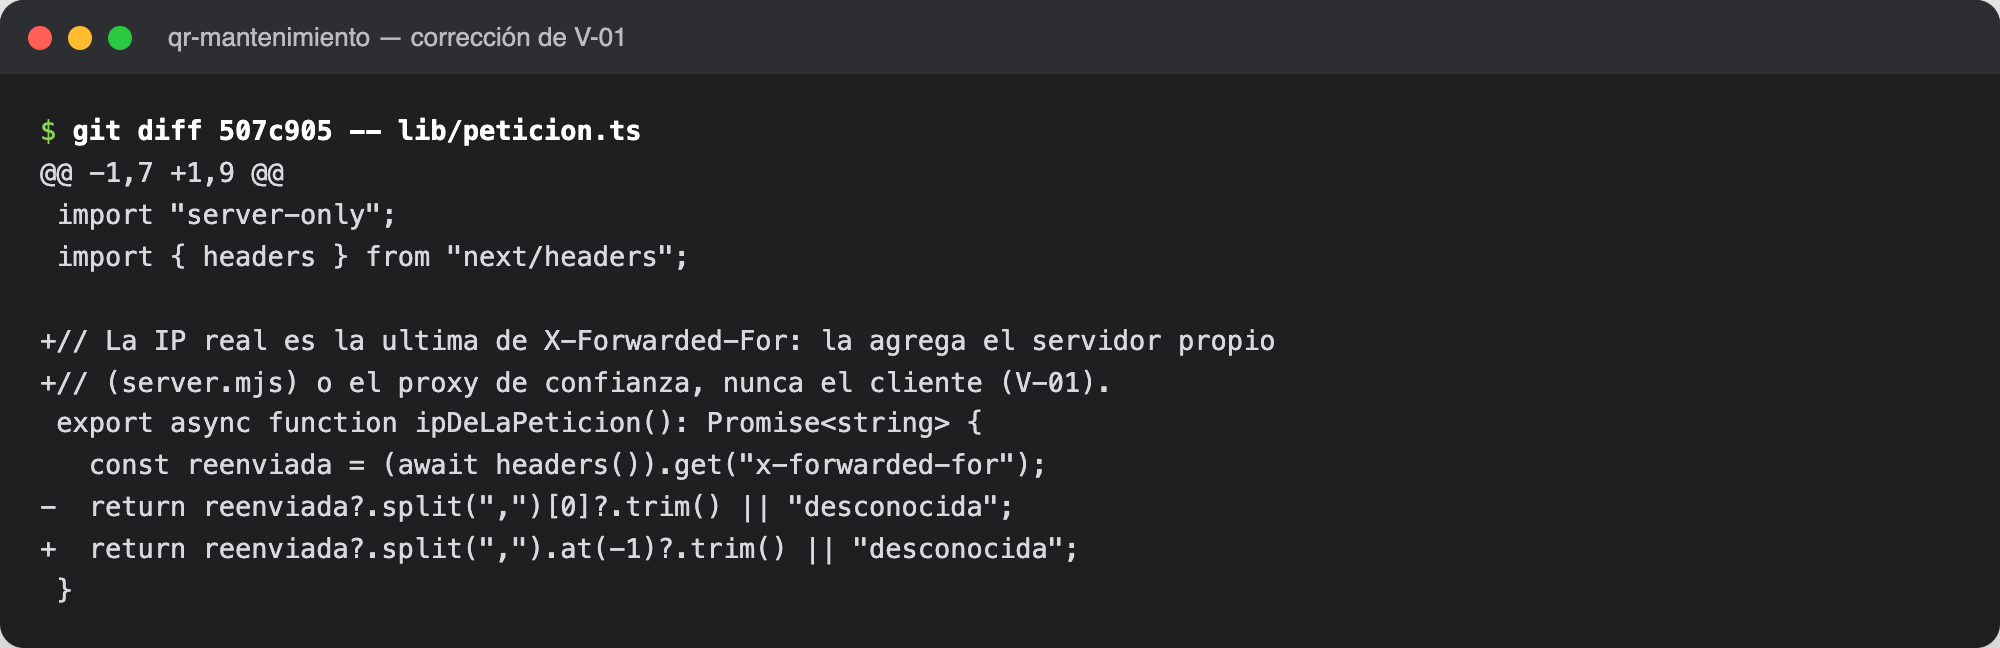
\includegraphics[width=\linewidth]{img/07-correccion-v01.png}
  \caption{Cambio en la función que obtiene la IP del cliente.}
  \label{fig:v01}
\end{figure}

Después de la corrección, la bitácora registra la dirección real de todos los intentos y ninguna de las 25 direcciones inventadas de la prueba P-38 (figura \ref{fig:bitacora-real}).

\begin{figure}[H]
  \centering
  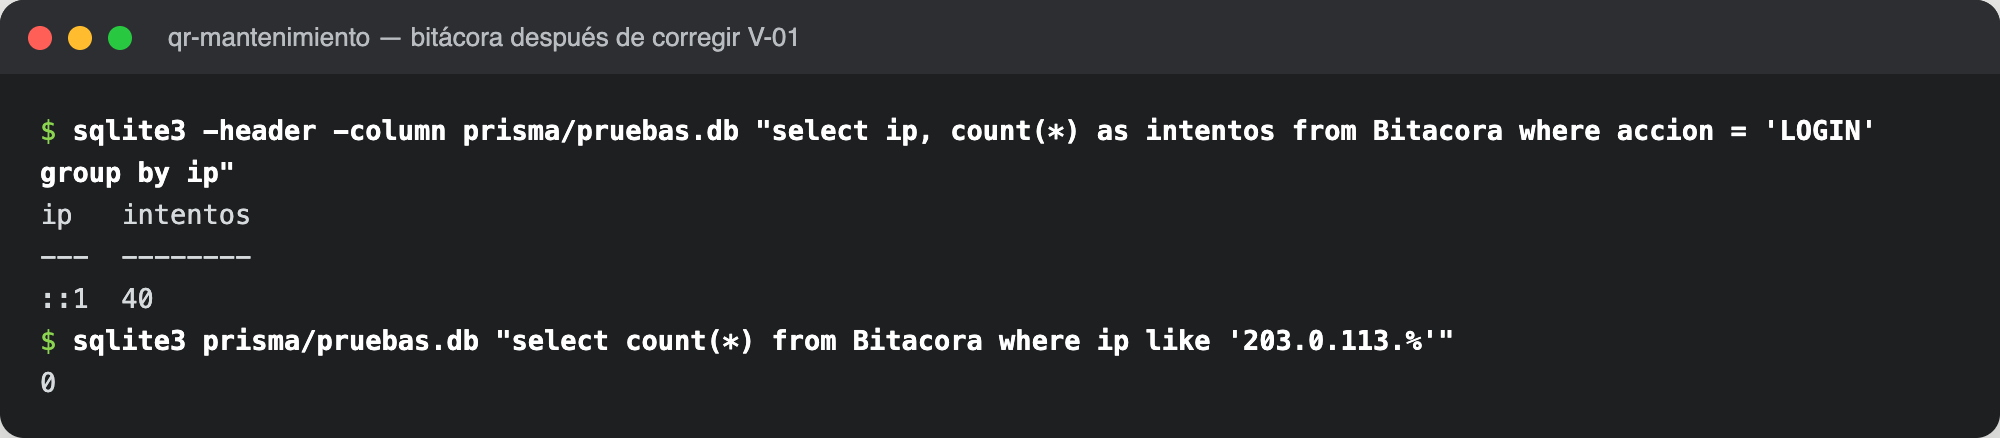
\includegraphics[width=\linewidth]{img/07-bitacora-ip-real.png}
  \caption{La bitácora guarda solo la dirección real después de corregir V-01.}
  \label{fig:bitacora-real}
\end{figure}

\subsection{V-02. Asignaciones de días pasados}

La restricción ya existía en la pantalla, así que la llevamos también al servidor. La función que quita una asignación ahora revisa la fecha y rechaza las de días pasados con un mensaje claro. Como segunda barrera, la consulta que borra la asignación incluye la condición de fecha, de modo que aunque se saltara la primera revisión no borraría nada del pasado (figura \ref{fig:v02}).

\begin{figure}[H]
  \centering
  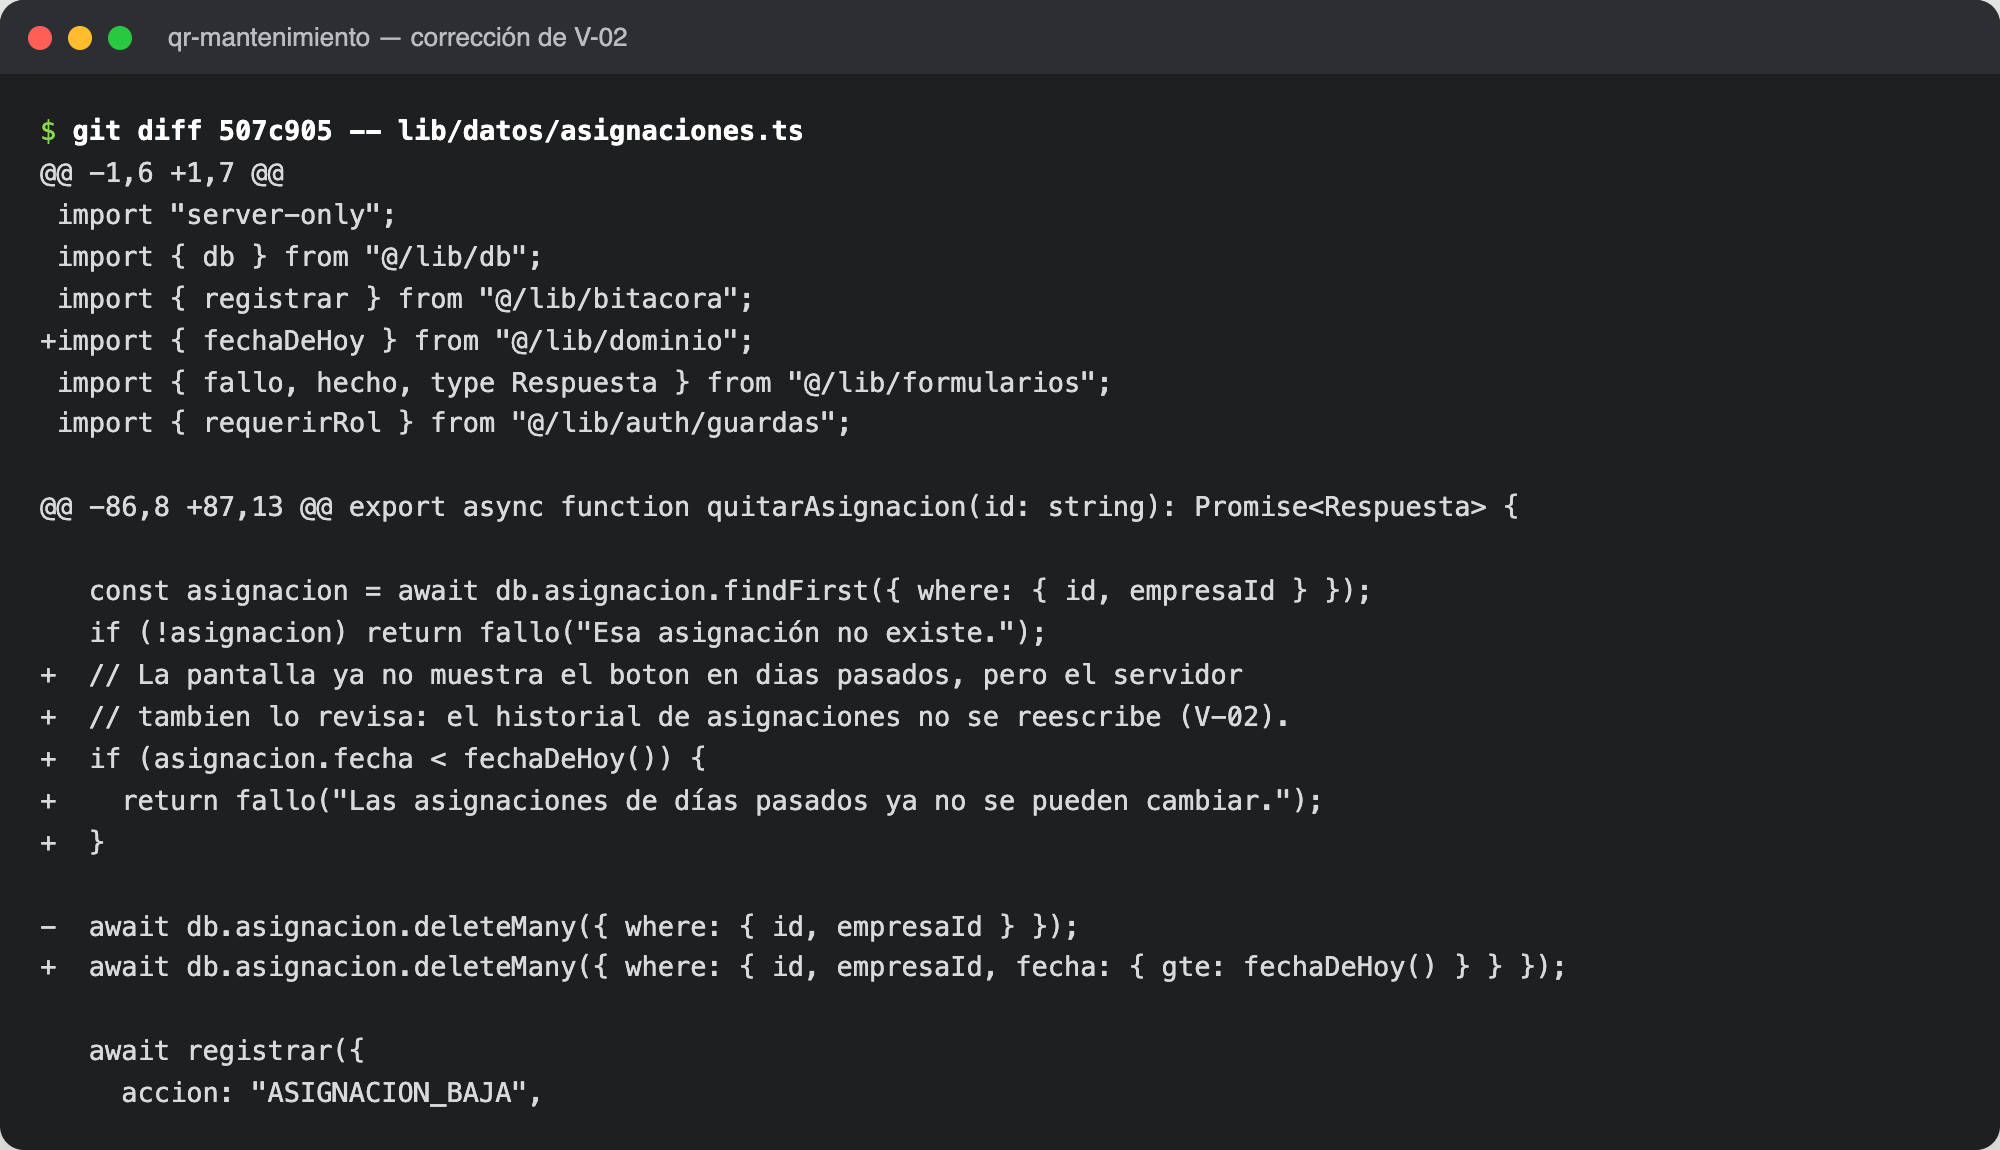
\includegraphics[width=\linewidth]{img/07-correccion-v02.png}
  \caption{Revisión de la fecha en la función que quita asignaciones.}
  \label{fig:v02}
\end{figure}

\subsection{V-03 a V-07. Librerías vulnerables}

Las vulnerabilidades de las librerías las corregimos actualizando versiones. En cada caso elegimos la solución que eliminaba la vulnerabilidad sin romper el sistema.

\begingroup\small\setlength{\tabcolsep}{4pt}\renewcommand{\arraystretch}{1.25}
\begin{longtable}{L{0.22}L{0.15}L{0.15}L{0.40}}
\toprule
\textbf{Librería} & \textbf{Antes} & \textbf{Después} & \textbf{Cómo y por qué} \\
\midrule
\endfirsthead
\toprule
\textbf{Librería} & \textbf{Antes} & \textbf{Después} & \textbf{Cómo y por qué} \\
\midrule
\endhead
\bottomrule
\endfoot
vitest y tinypool (V-03, V-05) & vitest 3.2.7 & vitest 5.1.2 & Actualizamos el ejecutor de pruebas a la versión más reciente, que ya trae una versión corregida de tinypool. Requirió actualizar también los tipos de Node.js a la versión 24. \\
deepmerge-ts (V-04) & 7.1.5 & 8.0.2 & Corregirlo con npm audit implicaba pasar a Prisma 7, un cambio mayor que modifica cómo se conecta a la base. En su lugar forzamos la versión corregida dentro de Prisma 6 con la opción \texttt{overrides} de npm. \\
effect (V-04) & 3.21.0 & 3.22.5 & Igual que la anterior, con \texttt{overrides}. Comprobamos que Prisma siga generando el cliente y aplicando migraciones. \\
minimatch (V-06) & 7 a 11.0.0 & 11.0.9 & Se actualizó con \texttt{npm audit fix}, sin cambios de versión mayor. \\
shadcn (V-07) & Producción & Desarrollo & La movimos a las dependencias de desarrollo, que es donde corresponde, porque solo se usa para crear componentes. \\
\end{longtable}
\endgroup

Al revisar las dependencias otra vez encontramos algo que no esperábamos: \texttt{puppeteer-core}, la librería que agregamos para automatizar las pruebas dinámicas y generar las imágenes de evidencia, traía 9 vulnerabilidades altas en su versión 24. Es decir, la herramienta que usamos para probar la seguridad había agregado sus propios riesgos. La actualizamos a la versión 25.19.0, que las corrige. Esto nos recordó que las herramientas de desarrollo también hay que revisarlas.

\begin{figure}[H]
  \centering
  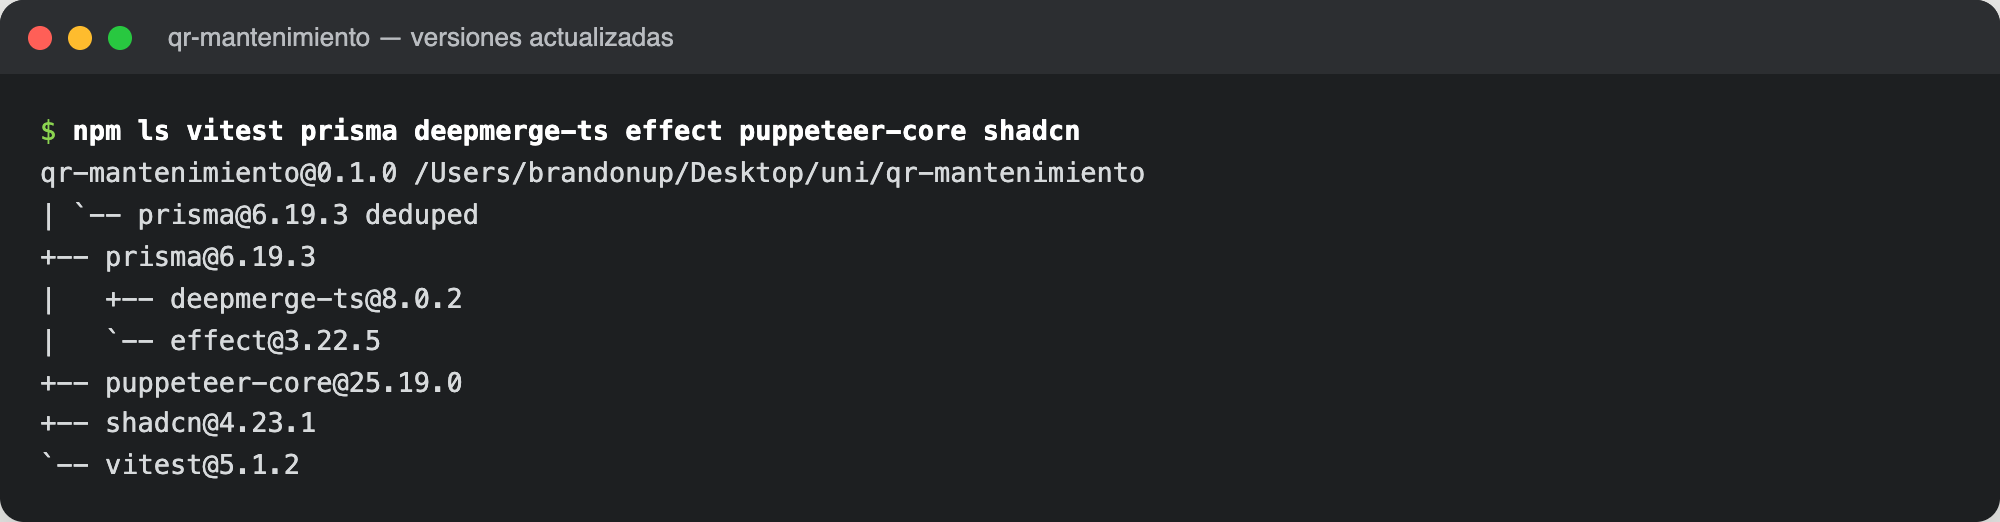
\includegraphics[width=\linewidth]{img/07-versiones.png}
  \caption{Versiones instaladas después de actualizar.}
  \label{fig:versiones}
\end{figure}
\begin{figure}[H]
  \centering
  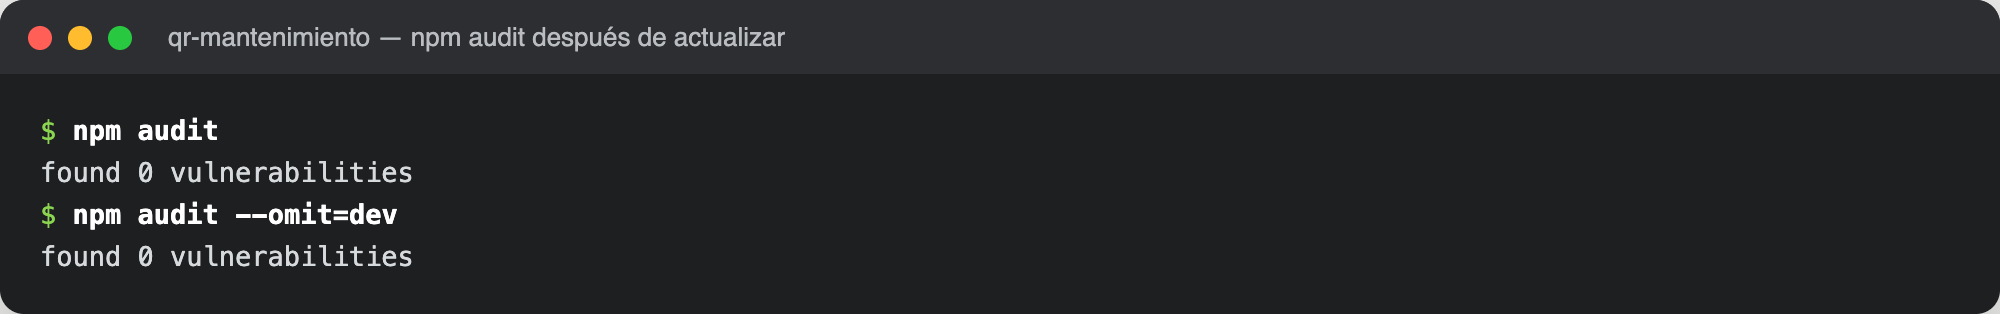
\includegraphics[width=\linewidth]{img/07-npm-audit.png}
  \caption{npm audit sin vulnerabilidades después de las correcciones.}
  \label{fig:audit-final}
\end{figure}

\subsection{Revalidación}

Después de corregir, repetimos todas las verificaciones en el mismo entorno de pruebas de la sección 4, con una base de datos nueva. Las 38 pruebas dinámicas pasaron, incluidas P-17 y P-38, que antes fallaban (figura \ref{fig:antes-despues}). En la prueba P-38 se bloquearon 14 de los 25 intentos: los primeros 11 todavía cabían en el límite de 20 fallos por dirección, porque la misma dirección ya llevaba 9 fallos de las pruebas anteriores, y a partir de ahí todos se rechazaron. Los resultados completos están en \nolinkurl{evidencias/07-correccion-y-revalidacion/resultados-revalidacion.json}.

\begin{figure}[H]
  \centering
  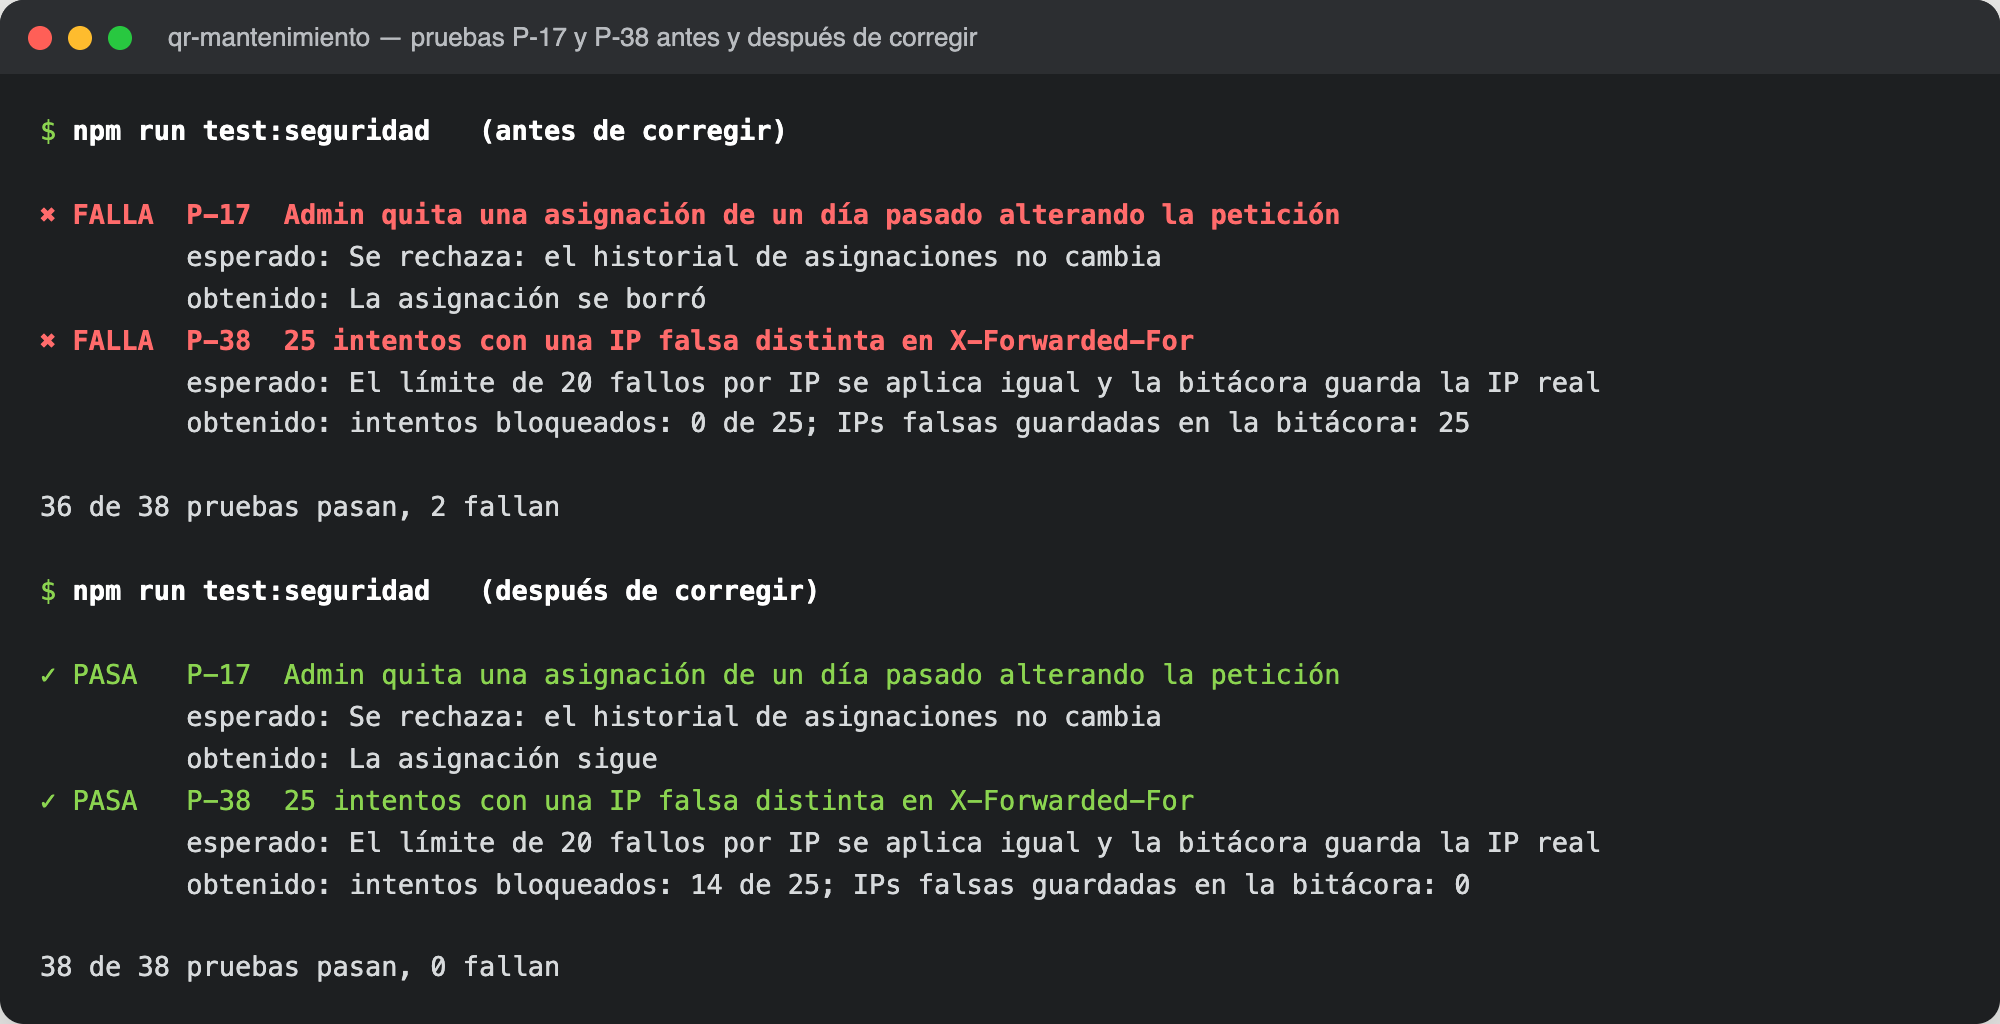
\includegraphics[width=\linewidth]{img/07-pruebas-antes-despues.png}
  \caption{Pruebas P-17 y P-38 antes y después de corregir.}
  \label{fig:antes-despues}
\end{figure}

También comprobamos que las correcciones no rompieran nada más: el análisis de ESLint y de TypeScript sigue limpio y las pruebas unitarias pasan (figura \ref{fig:calidad}).

\begin{figure}[H]
  \centering
  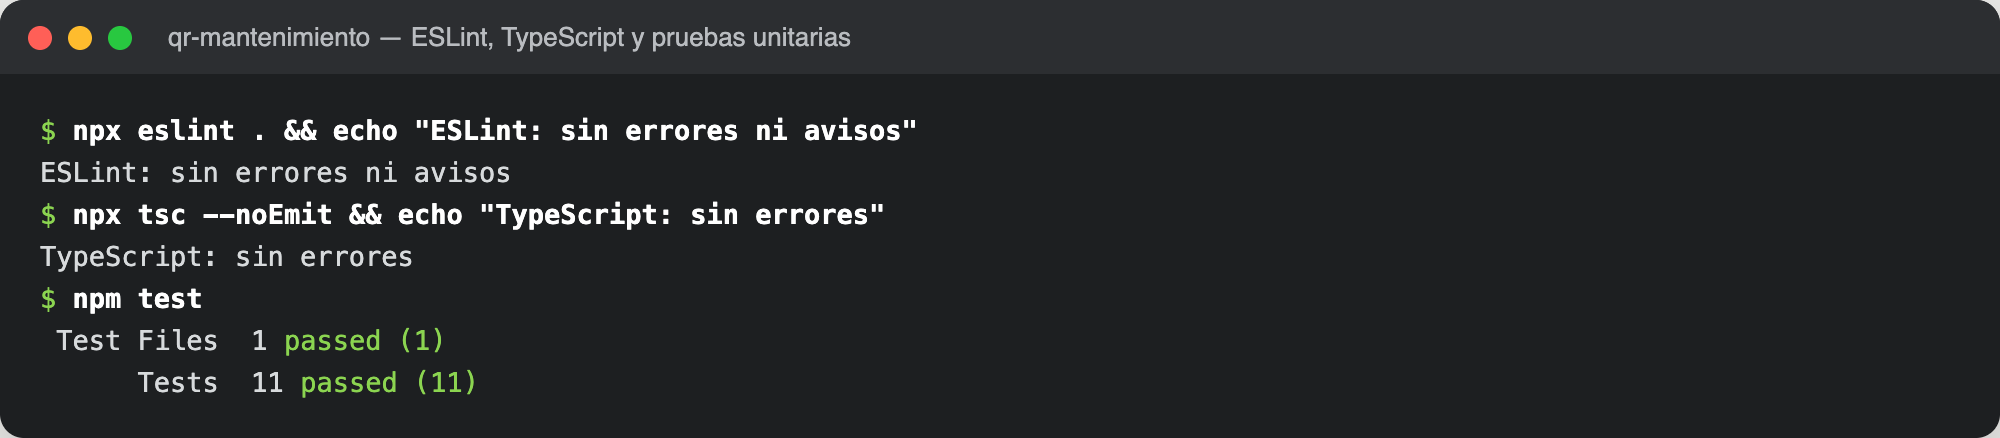
\includegraphics[width=\linewidth]{img/07-calidad.png}
  \caption{ESLint, TypeScript y pruebas unitarias después de corregir.}
  \label{fig:calidad}
\end{figure}
\begingroup\small\setlength{\tabcolsep}{4pt}\renewcommand{\arraystretch}{1.25}
\begin{longtable}{L{0.08}L{0.30}L{0.30}L{0.12}L{0.12}}
\toprule
\textbf{ID} & \textbf{Corrección} & \textbf{Cómo se revalidó} & \textbf{Antes} & \textbf{Después} \\
\midrule
\endfirsthead
\toprule
\textbf{ID} & \textbf{Corrección} & \textbf{Cómo se revalidó} & \textbf{Antes} & \textbf{Después} \\
\midrule
\endhead
\bottomrule
\endfoot
V-01 & Servidor propio que fija la IP real & Prueba P-38 y consulta a la bitácora & Falla & Pasa \\
V-02 & Revisión de fecha en el servidor & Prueba P-17 & Falla & Pasa \\
V-03 & vitest 5.1.2 & npm audit & Crítica & Sin hallazgos \\
V-04 & overrides de deepmerge-ts y effect & npm audit & Alta & Sin hallazgos \\
V-05 & vitest 5.1.2 & npm audit & Moderada & Sin hallazgos \\
V-06 & minimatch 11.0.9 & npm audit & Moderada & Sin hallazgos \\
V-07 & shadcn en desarrollo & npm audit solo de producción & Moderada & Sin hallazgos \\
\end{longtable}
\endgroup

\section{7. Verificación de requisitos y mitigación de amenazas}

\textit{Sección en desarrollo.}

\section{8. Integración continua y automatización}

\textit{Sección en desarrollo.}

\section{9. Dependencias y mecanismos criptográficos}

\textit{Sección en desarrollo.}

\section{10. Conclusiones}

\textit{Sección en desarrollo.}

% ═══════════════════════════ REFERENCIAS ═════════════════════════════════════
\newpage
\begin{thebibliography}{9}
\setlength{\itemsep}{5pt}

\bibitem{eslintsec} eslint-community. (s.f.). \textit{eslint-plugin-security}. GitHub. \url{https://github.com/eslint-community/eslint-plugin-security}

\bibitem{npmaudit} npm. (s.f.). \textit{npm-audit}. npm Docs. \url{https://docs.npmjs.com/cli/commands/npm-audit}

\bibitem{ghsa} GitHub. (s.f.). \textit{GitHub Advisory Database}. \url{https://github.com/advisories}

\bibitem{xff} Mozilla. (s.f.). \textit{X-Forwarded-For}. MDN Web Docs. \url{https://developer.mozilla.org/en-US/docs/Web/HTTP/Headers/X-Forwarded-For}

\bibitem{asvs} OWASP Foundation. (2021). \textit{OWASP Application Security Verification Standard}. \url{https://owasp.org/www-project-application-security-verification-standard/}

\bibitem{cwe} MITRE. (s.f.). \textit{CWE: Common Weakness Enumeration}. \url{https://cwe.mitre.org/}

\bibitem{owasp10} OWASP Foundation. (2021). \textit{OWASP Top 10:2021}. \url{https://owasp.org/Top10/}

\end{thebibliography}
\end{document}
